% !TeX root = chapter3_2d_ixaru.tex
% !TeX root = thesis.tex
\ifdefined\UtilIncluded
  \renewcommand{\startchapter}[1]{}
  \renewcommand{\stopchapter}{}
  \renewcommand{\undefinedlabel}[2]{}
\else

\newcommand{\startchapter}[1]{\begin{document}\setcounter{chapter}{#1}\addtocounter{chapter}{-1}}
\newcommand{\stopchapter}{\printbibliography[title=Bibliography,heading=bibintoc]\end{document}}


\documentclass{book}
\usepackage[utf8]{inputenc}


\usepackage{geometry}
\geometry{
  papersize={170mm,240mm},
}

\usepackage{amsfonts,amsmath, amsthm, amssymb, mathtools}
\usepackage{xspace}
\usepackage[hidelinks,bookmarks,pdfusetitle]{hyperref}
\usepackage{listings}
\usepackage[pdftex]{graphicx}
\usepackage{bm}
\usepackage[english]{babel}
\usepackage{caption}
\usepackage{subcaption}
\usepackage[usenames,dvipsnames]{xcolor}
\usepackage{physics}
\usepackage{multicol}
\usepackage{xstring}
\usepackage{pythonhighlight}
\usepackage{parskip}
\usepackage{thmtools}
\usepackage{relsize}
\usepackage{bookmark}
\usepackage{lmodern}
\usepackage{ifthen}
\usepackage{biblatex}
\usepackage{microtype}
\usepackage{csquotes}
\usepackage{numprint}
\usepackage{mleftright}
\npthousandsep{{\ifmmode\mskip2mu\else\hskip0.2em\fi}}
\npdecimalsign{.}

\addbibresource{references.bib}

\newtheorem{theorem}{Theorem}[chapter]
\newtheorem{lemma}[theorem]{Lemma}
\newtheorem{corollary}[theorem]{Corollary}
\newtheorem{definition}[theorem]{Definition}

\DeclareRobustCommand{\oneD}{{1{\relsize{-1}D}}\xspace}
\DeclareRobustCommand{\twoD}{{2{\relsize{-1}D}}\xspace}
\DeclareRobustCommand{\threeD}{{3{\relsize{-1}D}}\xspace}
\DeclareRobustCommand{\cpp}{{{C\nolinebreak[4]\hspace{-.05em}\raisebox{.4ex}{\relsize{-3}\textbf{++}}}\xspace}}
\pdfstringdefDisableCommands{%
  \def\cpp{C++}%
  \def\oneD{1D}%
  \def\twoD{2D}%
  \def\threeD{3D}%
}

\newcommand{\longchapter}[2][]{%
  \chapter[#2]{#2}%
  \ifthenelse{\equal{#1}{}}{}{\chaptermark{#1}}}

\newcommand{\NN}{\mathbb{N}}
\newcommand{\ZZ}{\mathbb{Z}}
\newcommand{\QQ}{\mathbb{Q}}
\newcommand{\QQbar}{\overline{\mathbb{Q}}}
\newcommand{\RR}{\mathbb{R}}
\newcommand{\CC}{\mathbb{C}}

\newcommand{\Eigen}{\texttt{Eigen}}

\newcommand{\sage}{\texttt{sage}\xspace}

\newcommand{\hamiltonian}{\mathcal{H}}

\newcommand{\transposesign}{\intercal}
\newcommand{\transpose}[1]{{#1}^\transposesign}
\newcommand{\adjointsign}{\text{H}}
\newcommand{\adjoint}[1]{{#1}^\adjointsign}

\newcommand{\xmin}{{x_{\text{min}}}}
\newcommand{\xmax}{{x_{\text{max}}}}
\newcommand{\ymin}{{y_{\text{min}}}}
\newcommand{\ymax}{{y_{\text{max}}}}

\newcommand{\Cbottom}{\vb{C}_\text{bottom}}
\newcommand{\Ctop}{\vb{C}_\text{top}}
\newcommand{\ubottom}{\vb{u}_\text{bottom}}
\newcommand{\utop}{\vb{u}_\text{top}}

\DeclareMathOperator{\diag}{diag}
\DeclareMathOperator{\tridiag}{tridiag}
\DeclareMathOperator{\eigs}{eigs}
\DeclareMathOperator*{\argmin}{arg\,min}
\DeclareMathOperator{\Ai}{Ai}
\DeclareMathOperator{\Bi}{Bi}
\DeclareMathOperator{\OO}{\mathcal{O}}

% https://tex.stackexchange.com/a/18192/163747
\makeatletter
\newcommand{\undefinedlabel}[2]{%
  \protected@write \@auxout {}{\string \newlabel {#1}{{#2}{\thepage}{#2}{#1}{}} }%
  \hypertarget{#1}{}
}
\makeatother

\fi
\gdef\UtilIncluded{}


\startchapter{3}

\undefinedlabel{cha:c2}{2}
\undefinedlabel{cha:c4}{4}
\undefinedlabel{the:c2_slp_countable}{2.x}
\undefinedlabel{the:c2_kth_eigen_k_roots}{2.x}
\undefinedlabel{sec:c2_experiment_with_jumps}{2.x.x}

\longchapter[A shooting method]{A shooting method for the \twoD time-independent Schrödinger equation}\label{cha:c3}

There are many general purpose methods available for solving partial differential equations. Each method has its own benefits and disadvantages. As a rule of thumb one can say that a method which is very general and widely applicable, will be less efficient, or less accurate, or both than a method which is specifically tuned for the problem at hand. With that in mind, there is a real advantage to gain when investing time and research into a highly tuned optimized method for a specific problem.

In this, and the next, chapter we will study two-dimensional time-independent Schrödinger equations
\begin{equation}\label{equ:c3_schrodinger_2d}
  -\nabla^2\psi(x, y) + V(x, y) \psi(x, y) = E \psi(x, y)
\end{equation}
on the domain $\Omega = [\xmin, \xmax]\times[\ymin, \ymax]$. We will only consider homogeneous Dirichlet boundary conditions, this means $\forall (x, y) \in \dOmega : \psi(x, y) = 0$. The function $V: \RR^2 \to \RR$ is called the potential function. This potential, together with the domain and the boundary conditions, defines the Schrödinger problem. When \emph{solving} the time-independent Schrödinger equation, one is searching for values for $E$ for which a function $\psi(x, y)$  exists such that they together satisfy the Schrödinger problem \eqref{equ:c3_schrodinger_2d}. Such a value $E$ is called an \emph{eigenvalue} corresponding to the \emph{eigenfunction} $\psi(x, y)$.

From a functional analysis perspective, the Schrödinger problem can also be interpreted as finding the eigenvalues and eigenfunctions of the \emph{Hamiltonian} $\hamiltonian$, this is the linear functional operator:
$$
  \hamiltonian := -\nabla^2 + V(x, y)\text{,}
$$
defined on the domain $\Omega$ with given boundary conditions.

Theoretically, working within the functional analysis framework is extremely useful. Many powerful results are available for all kinds of operators on all kinds of domains. In our case we are interested in self-adjoint elliptic operators, for if $V(x, y)$ is bounded and continuous then the Hamiltonian is self-adjoint and elliptic. Proving this here is non-trivial. Not because it is a particular difficult proof, in some textbooks this is merely an example of proven theorems. But all proofs require a thoroughly developed functional analysis framework. As an example of this framework: in the series of books starting with \cite{reed_functional_1980}, the authors start with defining functional spaces and provide some basic topological ideas to finally, after almost 200 pages, define a functional operator. It takes another 50 pages before they consider the spectrum of such an operator. So, in these 250 pages they were able to very rigorously define the needed concepts. Only in the fourth volume \cite{reed_iv_1978}, all parts of the puzzle are available to prove the Hamiltonian operator is self-adjoint. This self-adjointness in turn implies many theorems proven in volume two \cite{reed_ii_1975}.

Even though numerical methods are able to take a few theoretical shortcuts\footnote{For example, if we numerically approximate the integral $\int_a^b f(x)\,\dd x$ we use our favorite quadrature rule and plugin the function $f$. We are not concerned if $f$ is sufficiently integrable. We are not concerned that $f$ could be not \emph{almost everywhere} continuous. The only thing we need is to be able to evaluate $f$ in the points required by the quadrature rule.}, having a thorough understanding of the theory can be quite instructive. For now, we will not provide the functional analysis background, or rigorous proofs for the properties of Hamiltonian operators. However, we will state some useful theorems specifically for the Schrödinger problem at hand. The theorems we provide here are all special cases of more general results from functional analysis, proofs for these can be found in many textbooks, for example \cite{reed_functional_1980} and other books in the series.

But first let us define a \emph{regular} Schrödinger problem\footnote{The definition we provide here is only for two-dimensional problems. Changing the number of dimensions will not alter the provided theorems.} to be equation \eqref{equ:c3_schrodinger_2d} defined on a bounded Lipschitz\footnote{Formally, a Lipschitz domain has a Lipschitz continuous boundary. Intuitively, a Lipschitz domain has a ``sufficiently regular" boundary. \cite{dacorogna_introduction_2008}} domain $\Omega \subseteq \RR$ with linear, real and continuous boundary conditions and let $V(x, y) : \Omega \to \RR$ be continuous (and therefore bounded) on $\Omega$. With this in hand, we can state analogous theorems as in the one-dimensional case.

\begin{theorem}\label{the:c3_real_eigenvalues}
  All eigenvalues of a regular Schrödinger problem are real. Corresponding eigenfunctions can always be scaled such that they are real.
\end{theorem}

This first theorem states that to find solutions no complex numbers are necessary. This significantly simplifies an implementation of a method.

\begin{theorem}\label{the:c3_eigs_countable}
  The number of eigenvalues of a regular Schrödinger problem are countable. All eigenvalues have a lower bound and no upper bound. This implies that these can be written as:
  $$
    E_0 \leq E_1 \leq E_2 \leq \dots \to \infty \text{.}
  $$
\end{theorem}

Note that in contrast to theorem \ref{the:c2_slp_countable}, eigenvalues are no longer guaranteed to be simple. With this we mean that for the same eigenvalue, multiple linear independent eigenfunctions can be found. Such eigenvalues are said to be degenerate. If the corresponding eigenfunction space has dimension $3$, for example, the eigenvalue is said to have multiplicity three.

The last theorem we provide for now will give some information about the eigenfunctions.

\begin{theorem}\label{the:c3_eigs_othogonal}
  For two different eigenvalues $E_m$ and $E_n$, the corresponding eigenfunctions $\psi_m(x, y)$ and $\psi_n(x, y)$ will be orthogonal on $\Omega$.

  $$
    \int_\omega \psi_m(\vb{x}) \psi_n(\vb{x}) \, \dd \vb{x} = 0 \quad \text{ if $E_m \neq E_n$.}
  $$
\end{theorem}

These theorems give a very clear picture about what a solution will look like. But also what kind of questions we want to be able to handle, for example: ``What is the smallest eigenvalue?'', or ``Draw a graph of the first few eigenfunctions.''. To put these theorems in context we consider the following example.

\begin{figure}
  \begin{center}
    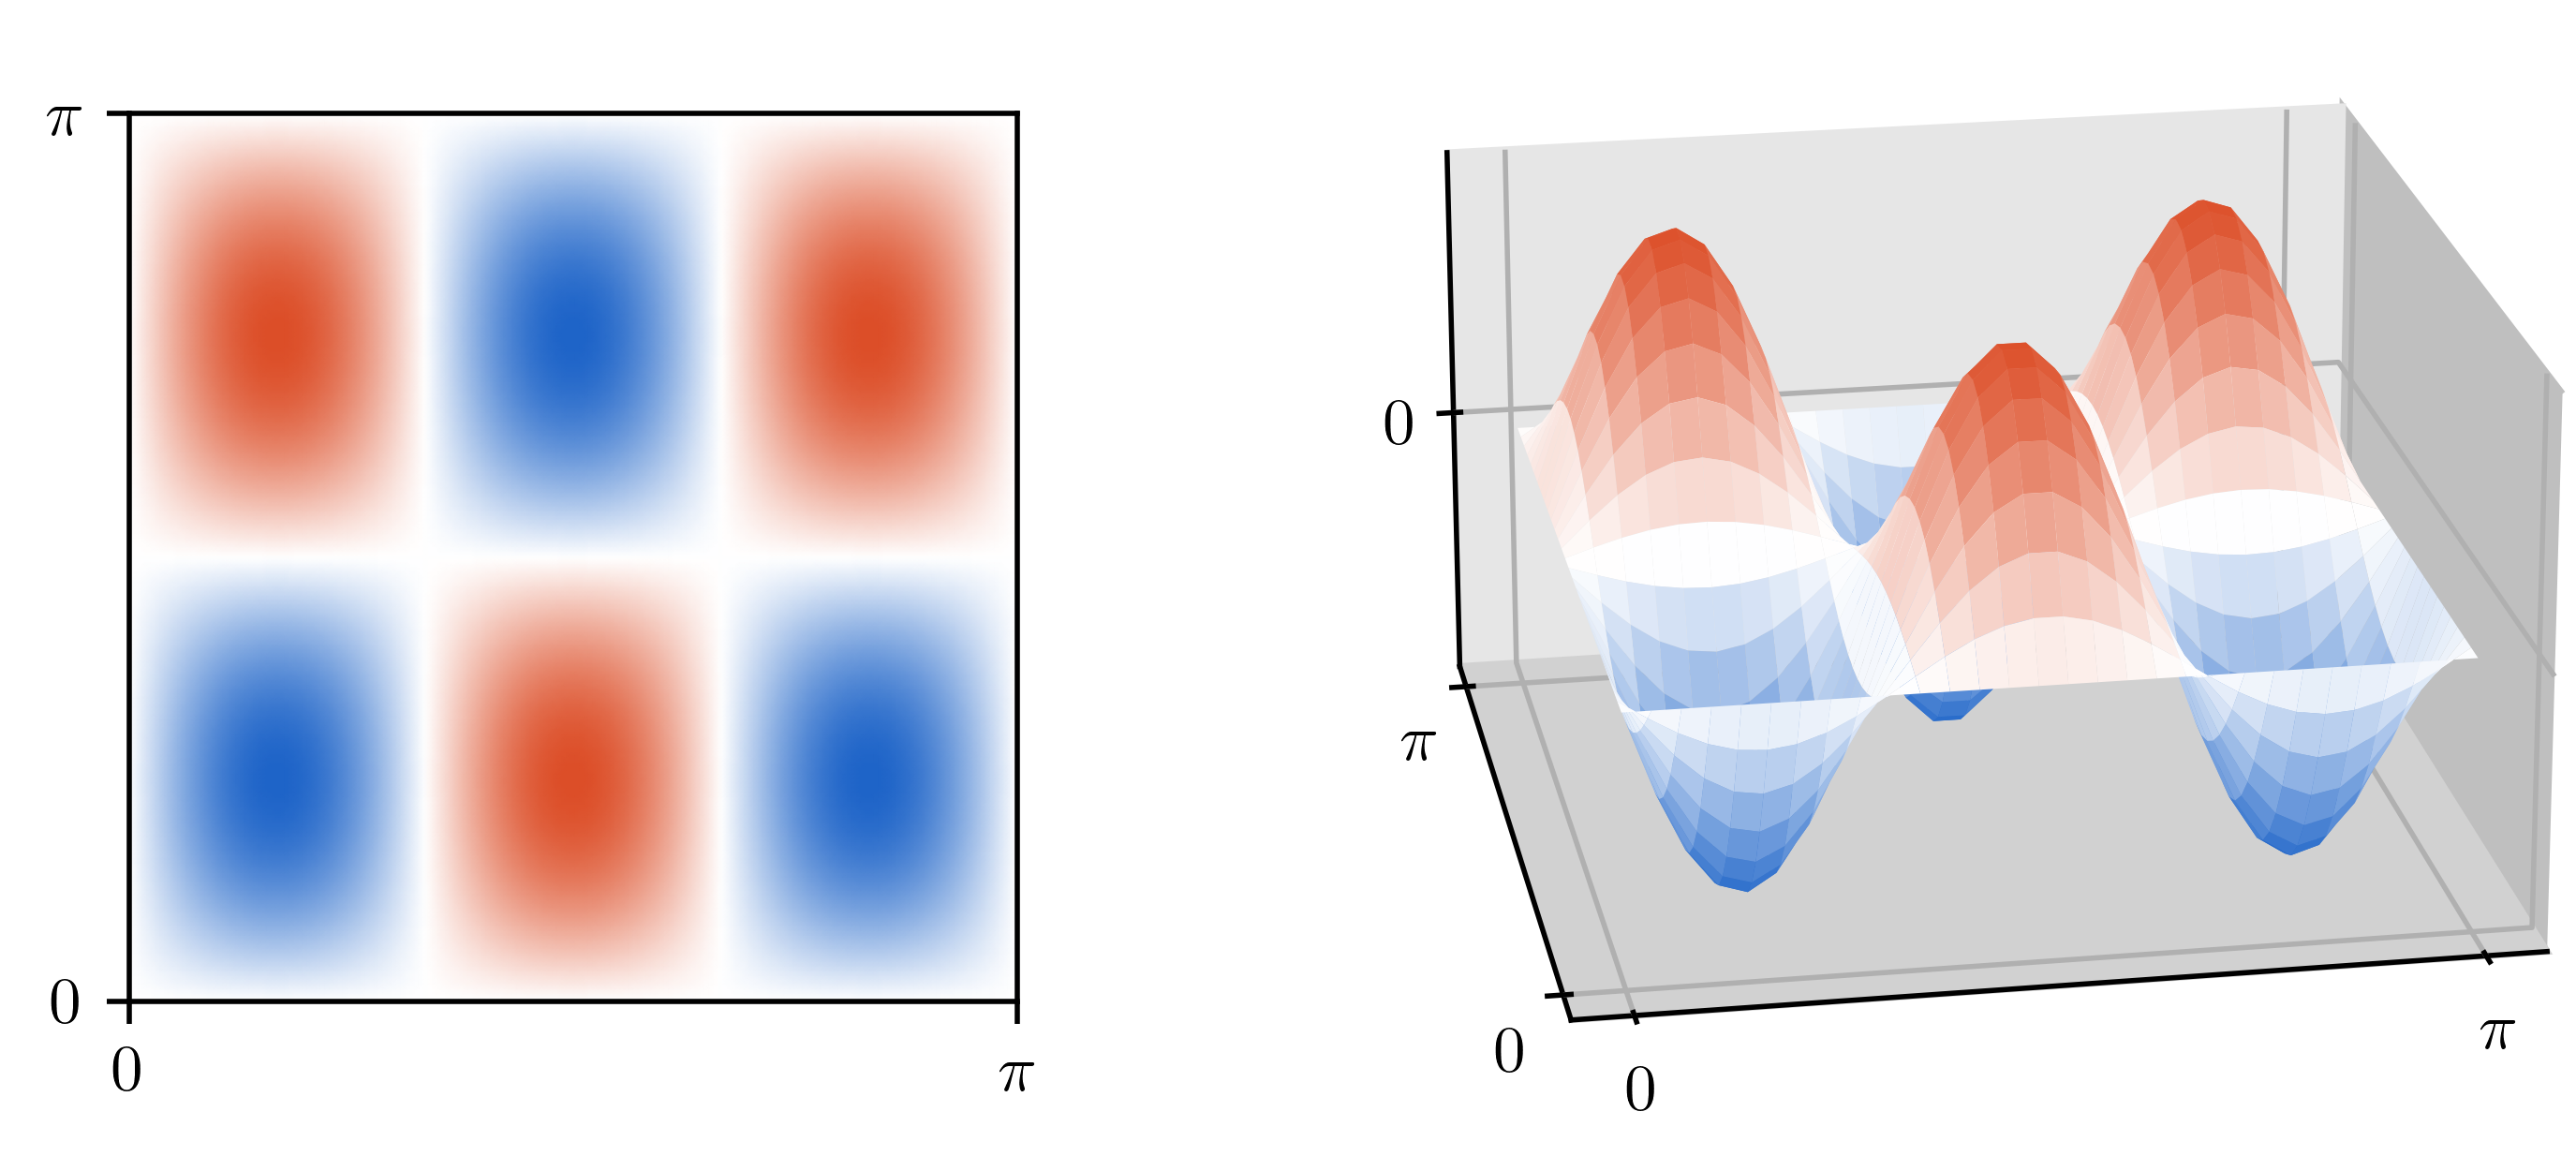
\includegraphics[width=\textwidth]{img/chapter3/example_zero_both.png}
  \end{center}
  \caption{A 2D and 3D plot of the eigenfunction corresponding to $i = 3$ and $j = 2$ from equation \ref{equ:c3_zero_example_eigenfunctions}, the eigenvalue is $E_{3,2} = 13$.}\label{fig:example_zero}
\end{figure}

As an example we consider the Schrödinger problem on the domain $[0, \pi] \times [0, \pi]$ with homogeneous Dirichlet boundary conditions and zero potential. Its equation is given as
\begin{equation}\label{equ:c3_example_zero_potential}
  -\pdv[2]{\psi}{x} - \pdv[2]{\psi}{y} = E \psi(x, y)\text{.}
\end{equation}

Now we write an eigenfunction $\psi(x, y)$ as a $y$-dependent linear combination of the $x$-dependent functions $\sin(x)$, $\sin(2x)$, $\sin(3x)$, $\dots$ which satisfy the boundary conditions:
\begin{equation}\label{equ:c3_zero_example_sin_basis}
  \psi(x, y) = \sum_{i=1}^\infty c_i(y) \sin(ix)\text{.}
\end{equation}

Since $\{\sin(x), \sin(2x), \dots\}$ construct a basis for $L^2_0(\Omega)$, this is the space of compactly supported square integrable functions on $\Omega$, all possible eigenfunctions are expressed with equation \eqref{equ:c3_zero_example_sin_basis}. If we plug this into the Schrödinger equation then we get
$$
  \sum_{i=1}^\infty i^2 c_i(y) \sin(ix) - \sum_{i=1}^\infty \dv[2]{c_i}{y}(y) \sin(ix) = \sum_{i=1}^\infty E c_i(y) \sin(ix)\text{.}
$$
Linear combinations of basis functions can only be equal if their coefficients are equal, thus:
\begin{equation}\label{equ:c3_zero_example_ode}
  (i^2 - E) c_i(y) = \dv[2]{c_i}{y}(y) \quad \text{ with $c_i(0) = c_i(\pi) = 0$ for each $i \in \{1, 2, \dots\}$.}
\end{equation}
Define $j := \sqrt{E - i^2}$. The ordinary differential equation \eqref{equ:c3_zero_example_ode} will only have solutions if $j$ is a strictly positive integer, specifically: $c_i(y) = \sin\left(\sqrt{E-i^2} y\right)$. This implies that all eigenvalues of \eqref{equ:c3_example_zero_potential} are
$$
  E_{i, j} = i^2 + j^2 \quad \text{ for all $i, j \in \{1, 2, \dots\}$}
$$
with corresponding eigenfunction
\begin{equation}\label{equ:c3_zero_example_eigenfunctions}
  \psi_{i,j} = \sin(ix) \sin(jy)\text{.}
\end{equation}

The eigenvalues are summarized in the following table.

\begin{tabular}{ccccccc}
  \toprule
  $0$       & $1$,$2$             & $3$       & $4$,$5$             & \dots & $30$, $31$, $32$              & \dots \\
  \midrule
  $E_{1,1}$ & $E_{1,2} = E_{2,1}$ & $E_{2,2}$ & $E_{1,3} = E_{3,1}$ & \dots & $E_{1,7} = E_{5,5} = E_{7,1}$ & \dots \\
  $2$       & $5$                 & $8$       & $10$                & \dots & $50$                          & \dots \\
  \bottomrule
\end{tabular}

Here we see that there are many degenerate eigenvalues, the $30^\text{th}$ eigenvalue $50$ even has multiplicity three. And, the $234^\text{th}$ eigenvalue with value $325$ even has multiplicity six. With some number theory, one can prove that the multiplicity of an eigenvalue can be unbounded.

A visualization of the eigenfunctions is found in figure \ref{fig:example_zero}. Here we have visualized the surface in a three-dimensional plot on the right. For clarity, we will use most of the time the two-dimensional representation on the left. Note that no color-legend is provided in the two-dimensional representation, as eigenfunctions may always be scaled.

The eigenvalue corresponding to the eigenfunction from figure \ref{fig:example_zero} has multiplicity two. Another linear independent eigenfunction can be found by swapping $x$ and $y$.

For almost all potential functions $V$ however, the corresponding Schrödinger equation can not be solved symbolically. So when one is interested in solutions, one has to resort to numerical methods. When only the ground state, that is the lowest eigenvalue, or maybe only few of the lowest eigenvalues are required, general numerical methods may suffice. Some examples of such techniques are finite difference based methods, or a finite element analysis. When higher eigenvalues are required, the eigenfunctions become more and more oscillatory. For the one-dimensional problem we have seen that general methods have difficulties with highly oscillatory functions, these same difficulties are expected for two-dimensional problems. In chapter \ref{cha:c4} we will study such a more general method, and develop our own method.

This chapter is dedicated to the study and improvement of the method proposed in \cite{ixaru_new_2010} by Ixaru. In section \ref{sec:c3_ixarus_method}, we will follow \cite{ixaru_new_2010} and study the method itself. Later on, in section \ref{sec:c3_improvements} we will highlight some challenges with using this method, and propose some improvements. Section \ref{sec:c3_index_of_e} contains the new theory we have developed to determine the index of an eigenfunction. And lastly, in section \ref{sec:c3_experiments} some numerical experiments are presented.

\section{Ixaru's method}\label{sec:c3_ixarus_method}

The main idea of Ixaru's method is built on the well established technique (by among others Titchmarsh \cite{titchmarsh_eigenfunction_1962}) of writing a solution as a linear combination of well-chosen one dimensional basis functions $b_i(x)$: $\psi(x, y) = \sum_{i=1}^\infty b_i(x) c_i(y)$. A disadvantage of this known technique is that, to represent an eigenfunction along the whole of the domain, many basis functions are necessary to ensure accurate values. Ixaru mitigates this by proposing multiple sets of basis functions, depending on the position in the domain. More concretely, they suggest splitting the domain into $K$ different sectors along the $y$-axis\footnote{In the original article \cite{ixaru_new_2010}, the domain is split along the $x$-axis. But for notational purposes it is more convenient to split along the $y$-axis. Analogous for the 3d version of the method, the split would happen along the $z$-axis.}:
$$
  \ymin = y_0 < y_1 < y_2 < \dots < y_k < \dots < y_{K-1} < y_{K} = \ymax\text{.}
$$
This split in sectors is illustrated in figure \ref{fig:c3_2dsectors}.

\begin{figure}
  \begin{center}
    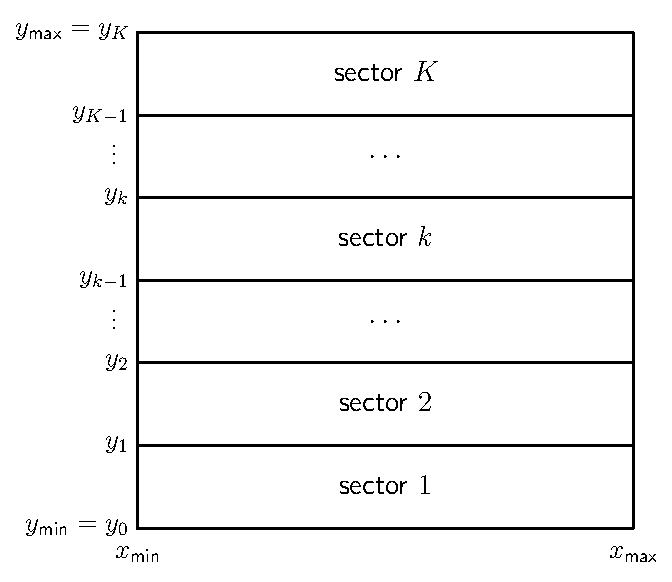
\includegraphics[width=.6\textwidth]{img/chapter3/2dsectors.pdf}
    \caption{\label{fig:c3_2dsectors} An illustration of the split in sectors along the $y$-axis for the domain $[\xmin, \xmax]\times[\ymin, \ymax]$.}
  \end{center}
\end{figure}

On each sector $k$ (with domain $[\xmin, \xmax]\times[y_{k-1}, y_k]$) a solution $\psi(x, y)$ will be approximated as a linear combination of $N$ basis functions:
\begin{equation}\label{equ:c3_lincomb_basis}
  \psi(x, y) \approx \sum_{i=1}^{N} b_i^{(k)}(x) c_i^{(k)}(y) = \transpose{{\vb{b}^{(k)}}}(x) \, \vb{c}^{(k)}(y) \text{.}
\end{equation}

Ideally, the used basis on sector $k$ should be related to the resulting eigenfunction on this sector. Of course, the eigenfunction is unknown, so using these, is not an option. In principle, there are many bases to choose from, a Fourier-basis is possible, or some basis based upon orthogonal polynomials. But, these well-known choices do not take advantage of the shape of the potential in the sector. In \cite{ixaru_new_2010}, the author proposes to use the eigenfunctions from the following one-dimensional Schrödinger problem:
\begin{equation}\label{equ:c3_one_dimensional_schrodinger}
  -\pdv[2]{b_i^{(k)}}{x} + \bar{V}^{(k)}(x)b_i^{(k)}(x) = \lambda_i^{(k)} b_i^{(k)}(x)
\end{equation}
with boundary conditions $b_i^{(k)}(\xmin) = b_i^{(k)}(\xmax) = 0$. The function $\bar{V}^{(k)}(x)$ is a constant (in the $y$-direction) approximation of the potential $V$ on the $k^\text{th}$ sector.

Using this basis is extremely promising. The basis functions are oscillatory for regions where $\bar{V}$ is small, and have an exponential behavior when $\bar{V}$ is large. This same behavior is expected for the two-dimensional eigenfunctions as well. For a potential function which becomes large, the two-dimensional eigenfunction is expected to be most present in the regions where $V(x, y)$ is small. The chosen one-dimensional basis functions $b_i^(k)(x)$ express this same behavior.

For the choice of $\bar{V}(x)$, in \cite{ixaru_new_2010} $\bar{V}^{(k)}(x) := V\left(x, \frac{y_{k-1} + y_k}{2}\right)$ is used. We will use this as well, for now. Later, we will remark that in some cases other choices may be beneficial.

Just like the constant perturbation methods for one-dimensional problems, this method employs shooting to locate the eigenvalues. To do this, for a fixed value of $E$, formulae are needed to propagate solutions from the bottom of the domain (along $y = \ymin$) upwards, and from the top of the domain ($y = \ymax$) downwards. So, given a solution at the beginning of sector $k$ expressed in the basis $b_i^{(k)}$: $ \psi(x, y_{k-1}) = \sum_{i=1}^{N} b_i^{(k)}(x)\, c_i^{(k)}(y_{k-1}) $, an expression is constructed to compute $c^{(k)}_i(y_k)$ at the end of the sector. Substituting \eqref{equ:c3_lincomb_basis} into \eqref{equ:c3_schrodinger_2d} using \eqref{equ:c3_one_dimensional_schrodinger} gives rise to

\begin{equation}\label{equ:c3_coupled_system}
  -\pdv[2]{\vb{c}^{(k)}}{y} + \vb{V}^{(k)}(y) \vb{c}^{(k)}(y) = E \vb{c}^{(k)}(y) \text{.}
\end{equation}

In this expression $\vb{V}^{(k)}$ is an $N\times N$ matrix depending on $y$:
\begin{equation}\label{equ:c3_v_matrix}
  \vb{V}^{(k)}_{ij}(y) = \int_{\xmin}^{\xmax} b_i^{(k)}(x) b_j^{(k)}(x) \left(V(x, y) - \bar{V}^{(k)}(x)\right) \dd x + \delta_{ij} \lambda_i^{(k)} \text{.}
\end{equation}

The system of ordinary differential equations given in \eqref{equ:c3_coupled_system} is a coupled system of Schrö\-dinger equations. For coupled systems, there are implementations of constant perturbation methods available \lilix{}\cite{ixaru_lilix_2002} or \matscs{}\cite{ledoux_numerical_2007} for example.

For the accurate computation of the integral in \eqref{equ:c3_v_matrix} we have developed specialized formulae. These will be presented later on in section \ref{sec:c3_calculate_vk}.

To be able to propagate a solution along the whole domain it is vital to have an expression to transfer solutions between consecutive sectors. Eigenfunctions should be continuous and continuously differentiable. To ensure this when transitioning between sectors we impose for all values $x \in [\xmin, \xmax]$:
\begin{align*}
  \transpose{\vb{b}^{(k)}}(x) \, \vb{c}^{(k)}(y_k)                   & =\, \transpose{\vb{b}^{(k+1)}}(x) \, \vb{c}^{(k+1)}(y_k)                            \\
  \text{and}\quad
  \transpose{\vb{b}^{(k)}}(x)\,\pdv{\vb{c}^{(k)}}{y}\left(y_k\right) & = \transpose{\vb{b}^{(k+1)}}(x)\,\pdv[]{\vb{c}^{(k+1)}}{y}\left(y_k\right) \text{.}
\end{align*}
Multiplying both sides with $\vb{b}^{(k)}(x)$ and integrating along the $x$-axis for each $i \in \{1, \dots, N\}$, gives
\begin{align*}
  \vb{c}^{(k+1)}(y_k)                       & = \vb{M}^{(k)} \vb{c}^{(k)}(y_k)                       \\
  \pdv[]{\vb{c}^{(k+1)}}{y}\left(y_k\right) & = \vb{M}^{(k)} \pdv[]{\vb{c}^{(k)}}{y}\left(y_k\right)
\end{align*}
with
$$
  \vb{M}^{(k)}_{ij} = \bra{b_{i}^{(k)}}\ket{b_{j}^{(k+1)}} = \int_\xmin^\xmax b_i^{(k)}(x) b_j^{(k+1)}(x) \dd x \text{.}
$$
Here we assumed the orthogonal basis $\left\{b_i^{(k)}(x)\right\}$ to be normalized $\bra{b_{i}^{(k)}}\ket{b_{j}^{(k)}} = \delta_{ij}$. In the infinite case this matrix $\vb{M}^{(k)}$ is orthogonal. In practice $N$ has to be finite, and $\vb{M}^{(k)}$ is in general no longer orthogonal. Intuitively this means that some information about the solution is lost when transitioning between sectors. This is a minor drawback, inherent to this method.

\todo{Visualize that $\vb{M}^{(k)}$ is no longer orthogonal.}

With these tools available, all that is left is to formalize how the shooting can be executed. Instead of propagating with a single starting condition (i.e. a column vector $\vb{c}^{(1)}(\ymin)$), all possible initial values (for homogeneous Dirichlet boundary conditions) are propagated at once. Therefore, we propose to start with:
$$
  \begin{matrix}
    \vb{C}^{(1)}(\ymin) = \vb{0}_{N\times N} &            & {\pdv[]{}{y}}\vb{C}^{(1)}(\ymin) = \vb{I}_{N\times N} \\
                                             & \text{and} &                                                                \\
    \vb{C}^{(K)}(\ymax) = \vb{0}_{N\times N} &            & {\pdv[]{}{y}}\vb{C}^{(K)}\left(\ymax\right) = \vb{I}_{N\times N}\text{.}
  \end{matrix}
$$

As we are using a multiple shooting procedure in the $y$-direction, the propagated values come together in a matching line $y = y_m$. Since eigenfunctions have to be continuous and continuously differentiable, a `matching' condition can be formulated.  Let us define $\Cbottom$ and $\Cbottom'$ to be the values of $\vb{C}^{(m)}(y_m)$ and ${\pdv[]{}{y}}\vb{C}^{(m)}\left(y_m\right)$ respectively when propagated from the bottom of the domain upwards. Analogous $\Ctop$ and $\Ctop'$ can be defined. Now the value $E$ is an eigenvalue of the original problem if and only if there exist vectors $\ubottom$ and $\utop$ such that
\begin{align}
  \Cbottom \cdot \ubottom                   & = \Ctop \cdot \utop           \nonumber \\
  \text{and }\quad \Cbottom' \cdot \ubottom & = \Ctop' \cdot \utop \text{.} \label{ref:c3_c1_matching}
\end{align}
In \cite{ixaru_new_2010}, $\Cbottom$ and $\Ctop$ are implicitly assumed to be non-singular. With this, equations \eqref{ref:c3_c1_matching} can be rearranged. This makes it equivalent with saying: $E$ is an eigenvalue of \eqref{equ:c3_schrodinger_2d} if and only if the mismatch matrix
\begin{equation}\label{equ:c3_psi_e}
  \vb{\Phi}(E) := \Cbottom'\Cbottom^{-1} - \Ctop'\Ctop^{-1}
\end{equation}
has a zero eigenvalue. Each linear independent eigenvector of $\vb{\Phi}(E)$ corresponding to eigenvalue $0$ implies a linear independent eigenfunction $\psi(x, y)$ of the Schrödinger equation. Conversely, each eigenfunction of the Schrödinger equation corresponding to $E$ will emit an eigenvector (corresponding to $0$) for \eqref{equ:c3_psi_e}. Therefore, the geometric multiplicity of the zero eigenvalue of this matrix is the same as the multiplicity of $E$ as an eigenvalue of \eqref{equ:c3_schrodinger_2d}. In the original article no details are provided about how one should find the values of $E$ for which the matrix $\vb{\Phi}(E)$ becomes singular. Later, in section \ref{sec:c3_locating_e}, we will present our method for finding those values. In section \ref{sec:c3_index_of_e}, we will go even further and demonstrate a technique which allows to determine the index of the eigenvalue in question.

This concludes our overview of the method described by Ixaru in \cite{ixaru_new_2010}. There are a few differences between our overview and the method as described in \cite{ixaru_new_2010}. Most notably, as stated in the beginning, we have swapped the roles of $x$ and $y$. Ixaru split the domain in sectors along the $x$-axis. To highlight the recursive nature of this method we have chosen to apply the split along the $y$-axis. To use this method for three-dimensional problems, we split the domain along the $z$-axis, and for the basis functions on each sector we solve the two-dimensional Schrödinger problem in the $x\,y$-plane. For each of these two-dimensional problems we split the domain along the $y$-axis, and solve some one-dimensional Schrödinger problems along the $x$-axis.

\section{Our improvements}\label{sec:c3_improvements}

As we have seen with the rise of constant perturbation methods for the one-dimensional Sturm-Liouville equation, research builds upon previous work. With this in mind we have identified some possibilities where Ixaru's method can be expanded or improved. This section follows primarily our work done in \cite{baeyens_fast_2020}.

We have made four large improvements and present them here in no particular order. First in section \ref{sec:c3_improvement_automatic_sectors}, we made the program able to automatically choose the optimal sector size, to ensure a provided tolerance. In section \ref{sec:c3_improvement_orthonormalization}, we were able to construct a formula to compute the inner product of two eigenfunctions. This formula allows us to normalized eigenfunctions, and construct an orthogonal basis of the eigenspace for degenerate eigenvalues. Section \ref{sec:c3_calculate_vk} is dedicated to the computation of the integral in equation \eqref{equ:c3_v_matrix}. And the last improvement we present here is a robust way to locate eigenvalues in section \ref{sec:c3_locating_e}. For this last improvement we had to develop some new theoretical results, which we will cover in section \ref{sec:c3_index_of_e}.

% Should we say something about scaling in between sectors?
% No, too much work, same idea as in MatSCS

\subsection{Automatic optimal sector size}\label{sec:c3_improvement_automatic_sectors}

When developing numerical methods (for any problem, not only for differential equations), it is most user-friendly to allow a user to only specify to which accuracy results are required. Everything else should be automatic. For example, an implementation of an adaptive quadrature rule should let the user specify only the function which to integrate, and the accuracy required. No extra parameters, such as the initial number of grid points or the order of the method for example, should be required\footnote{But ideally, a user who is experimenting or wants more control should be able to optionally specify some of these extra parameters.}. In \matslise{3} we have followed \matslise{2}, which has automatic sector size built in. It would improve the usability of this method if we could include something similar.


We could use the same ideas that \matslise{} is using, the only difference is the way we compute the error for a given sector. In the one-dimensional case, the difference between the 16th and 18th order propagation matrix is used to estimate the error. Here, we are propagating on each sector a coupled system of Schrödinger equations. This propagation is implemented with an adaptation of \matscs{} \cite{ledoux_numerical_2007}. In this adaptation two different propagation methods are implemented: a 10th order and 8th order method. The difference between the corresponding propagation matrices can be used to estimate the error that will be made on this sector.

In theory and in practice this works beautifully, but some optimizations are still possible. The selection algorithm works by guessing an initial sector size $s_0$. When the error is too large, a smaller sector size $s_1$ is chosen and the process starts over. One big disadvantage of this method is that when a sector was computed with an error that is too large, all computations are thrown away and everything is recomputed. This is quite wasteful when the sector size is only slightly adjusted. One of the things we can reuse are the basis functions. Initially these are computed as the solution of
$$
  -\pdv[2]{b_i}{x} + V(x, \bar{y}) = \lambda_i b_i
$$
with $\bar{y} = y_{k} + \frac{s_0}{2}$. But if $\frac{s_1}{2} \approx \frac{s_0}{2}$ then it is maybe not necessary to recompute these basis functions. In our testing we have seen that the algorithm is not very sensitive to when we decide $\frac{s_1}{2} \not\approx
  \frac{s_0}{2}$. We have chosen the heuristic that $y_k + \frac{s_1}{3} \leq \bar{y} \leq y_k + \frac{2 s_1}{3}$. Intuitively this means that we are happy with $\bar{y}$ as long as it is situated within the middle third of a sector. Another big advantage of not needing to recompute the basis functions is that the expensive recursive expressions, which we will see in section \ref{sec:c3_calculate_vk}, for the integrals $\int_{0}^{h} b_i(\delta)b_j(\delta)\delta^n \dd \delta $ can be reused.

\subsection{Orthonormalization of eigenfunctions}\label{sec:c3_improvement_orthonormalization}

For the one dimensional case, we know from theory that eigenfunctions corresponding to different eigenvalues are necessarily orthogonal. In theorem \ref{the:c3_eigs_othogonal} we have seen that eigenfunctions for different eigenvalues will always be orthogonal. But up to now, nothing has been stated about eigenfunctions corresponding to the same eigenvalue. For degenerate eigenvalues, the eigenspace will be multidimensional.

Ideally, the eigenfunctions returned by are program should form an orthonormal basis. For this we need to normalize eigenfunctions, and ensure that the returned basis of a multidimensional eigenspace is orthogonal. To execute normalization, the inner product $\bra{u}\ket{u} := \int_\Omega u^2$  of an eigenfunction $u$ with itself should be computed. To orthogonalize two linear-independent eigenfunctions in the same eigenspace, a Gram-Schmidt process can be used. For this process, there has to be a way to compute the inner product $\bra{u}\ket{v}$ of two functions $u$ and $v$ in this eigenspace.

To normalize an eigenfunction or to orthogonalize eigenfunctions, in both cases the inner product of two functions should be computable. One way would be to numerically estimate this value with some quadrature rules. In principle this is a valid approach, but in practice, this is quite computationally expensive. Therefore, we have constructed specialized formulae to compute these inner products:

\begin{theorem}
  Let $\psi_a(x, y)$ and $\psi_b(x, y)$ be two, not necessarily distinct, real eigenfunctions of the Schrödinger operator corresponding to the same eigenvalue $E$. Denote both eigenfunctions as linear combinations of one dimensional orthonormal basis functions (as described in section \ref{sec:c3_ixarus_method}, on a single sector).
  \begin{align*}
    \psi_a(x, y) = \transpose{\vb{b}(x)} \vb{c_a}(y) = \sum_i b_i(x) c_{a, i}(y) \\
    \psi_b(x, y) = \transpose{\vb{b}(x)} \vb{c_b}(y) = \sum_i b_i(x) c_{b, i}(y)
  \end{align*}
  On a rectangular domain $[\xmin, \xmax] \times [\ymin, \ymax]$ the inner product of these two functions can be expressed as:
  $$
    \bra{\psi_a}\ket{\psi_b} = \int_\xmin^\xmax \int_\ymin^\ymax \psi_a\psi_b \, \dd y \, \dd x = \left. \left(\pdv{\transpose{\vb{c_a}}}{E} \vb{c_b}' - \transpose{\vb{c_b}}\pdv{\vb{c_a}'}{E} \right) \right|_{y=\ymin}^{y=y_\ymax} \text{.}
  $$
  With $\vb{c_a}' = \dv[]{\vb{c_a}}{y}$, analogous for $\vb{c_b}' = \dv[]{\vb{c_b}}{y}$.
\end{theorem}
\begin{proof}
  By assumption $\psi_a$ and $\psi_b$ are solutions of the Schrödinger equation:
  \begin{align*}
    -\nabla^2 \psi_a + V \psi_a = E \psi_a \\
    -\nabla^2 \psi_b + V \psi_b = E \psi_b \text{.}
  \end{align*}
  Deriving the first equation with respect to $E$ and multiplying with $\psi_b$ gives
  \begin{align*}
    -\nabla^2\pdv{\psi_a}{E} \, \psi_b + V(x, y)\pdv{\psi_a}{E} \, \psi_b & = E \pdv{\psi_a}{E}\psi_b + \psi_a\psi_b \text{.} \\
    \intertext{The second equation can be multiplied with $ \pdv[]{\psi_a}{E}$ to result in}
    -\nabla^2\psi_b\,\pdv{\psi_a}{E}  + V(x, y)\psi_b\,\pdv{\psi_a}{E}    & = E \psi_b\pdv{\psi_a}{E} \text{.}
  \end{align*}
  The difference of these last two expressions can be integrated over the domain $[\xmin, \xmax]\times[\ymin, \ymax]$ to obtain an expression for the inner product $\bra{\psi_a}\ket{\psi_b}$. For brevity of notation we omit the integration boundaries, these are assumed to be the whole domain.

  \begin{align*}
    \iint \psi_a\,\psi_b = & \iint\nabla^2\psi_b\,\pdv{\psi_a}{E} - \iint \nabla^2\pdv{\psi_a}{E}\,\psi_b                                                               \\
    \intertext{The right-hand side can be calculated by applying Green's second identity:}
    \iint \psi_a\,\psi_b = & \oint \left(\pdv{\psi_a}{E} \nabla \psi_b \cdot \vb{n} -  \psi_b \nabla \pdv{\psi_a}{E} \cdot \vb{n} \right) \text{.}                      \\
    \intertext{This can be written explicitly on the integration domain as}
    \iint \psi_a\,\psi_b = & \left.\int_{\xmin}^{\xmax} \left(\pdv{\psi_a}{E} \pdv{\psi_b}{y} -  \psi_b \pdv[2]{\psi_a}{E}{y} \right) \dd x \right|_{y=\ymin}^{y=\ymax} \\
                           & +\left.\int_{\ymin}^{\ymax} \pdv{\psi_a}{E} \pdv{\psi_b}{x} \dd y \right|_{x=\xmin}^{x=\xmax} \text{.}                                     \\
    \intertext{Taking into account that the eigenfunctions $\psi_a$ and $\psi_b$ are expressed in terms of an orthonormal set of basis functions $\vb{b}(x)$, such that
      $$
        \int_{\xmin}^{\xmax} \vb{b}(x) \transpose{\vb{b}}(x) \dd x = \vb{I}_{n\times n} \text{,}
      $$
      we can simplify the expression to}
    \iint \psi_a\,\psi_b = & \left. \left(\pdv{\transpose{\vb{c_a}}}{E} \vb{c_b}' - \transpose{\vb{c_b}}\pdv{\vb{c_a}'}{E} \right) \right|_{y=\ymin}^{y=\ymax}          \\
                           & +\left.\int_{y_{k-1}}^{y_{k}} \pdv{\transpose{\vb{c_a}}}{E} \vb{b} \transpose{\vb{b}'} \vb{c_b} \dd y \right|_{x=\xmin}^{x=\xmax} \text{.}
  \end{align*}
  Since the basis functions satisfy the Dirichlet boundary conditions $\vb{b}(\xmin) = \vb{b}(\xmax) = \vb{0}$ the last term has to be zero, which proves the theorem.
\end{proof}

This theorem gives an expression for the inner product of two eigenfunctions on each sector. Summing these values across all sectors gives the inner product over the whole domain. This value, in turn, can be used to normalize an eigenfunction or orthogonalize different eigenfunctions for the same eigenvalue.

\subsection{Calculation of \texorpdfstring{$\vb{V}^{(k)}(y)$}{Vk(y)}}\label{sec:c3_calculate_vk}

Another improvement we have made can be found in the calculation of the matrix $\vb{V}^{(k)}(y)$ from equation \eqref{equ:c3_v_matrix}. When one wants to implement this definition accurately, some considerations have to be made. As the formula consist of an integral with a relatively complicated integrand, we have to consider in which points this integrand is known. Furthermore, evaluating more points is non-trivial.

In \cite{ixaru_new_2010}, they remark that not only the values of the basis function is known but also the values of their derivative. To use this, ideas from \cite{kim_quadrature_2002} are combined with the treatment of exponential fitting with two frequencies in \cite{ixaru_operations_1997}. This yielded a procedure close to \texttt{CENC1} from \cite{ixaru_exponential_2004}.

In our case, the story is quite different. Because of our improvements to Matslise, we can improve accuracy even further. In particular, the computation of $b_i^{(k)}(x)$ is now efficiently possible in arbitrary points. This allows us to use off-the-shelf adaptive quadrature rules, to ensure accuracy. As this was only a first test to approximate $\vb{V}^{(k)}(x)$, we did not use specialized exponentially fitted methods. When profiling our implementation we found that the time to execute these quadrature formulae was almost negligible.

So in practice, there was little need to improve even further, with more complicated quadrature formulae from \cite{ixaru_operations_1997,kim_quadrature_2002,conte_modified_2016}. But, as numerical analysts, we were still curious if some more fundamental improvements were possible. After all, the eigenfunctions $b_i^{(k)}(x)$, are approximated piecewise by a truncated series in the step size $\delta$ and the special functions $\eta_{-1}$, $\eta_{0}$, $\dots$ But also, the function $\bar{V}^{(k)}$ is already approximated by a sixteenth degree polynomial. The only `wildcard', so to speak, is the unknown general function $V(x, y)$, for a fixed value of $y$. In the middle of the $k^\text{th}$ sector, this function is approximated piecewise. As such, it is reasonable to assume, that a piecewise sixteenth degree polynomial can also be accurately fitted on this function $V(x, y)$, if the same pieces as for $\bar{V}^{(k)}$ are used.

More formal, let us split the interval $[\xmin, \xmax]$ into the same partition that \matslise{3} used to compute the basis functions: $\xmin = x_0, x_1, \dots, x_K = \xmax$. For a fixed value of $y$ on the section $[x_{l-1}, x_l]$, the potential $V(x, y)$ can be approximated by a sixteenth order polynomial, just like $\bar{V}^{(k)}(x)$. We thus approximate $V(x, y) - \bar{V}^{(k)}(x)$ on $x \in [x_{l-1}, x_l]$ by a polynomial $q_l(x)$. This means that to compute \eqref{equ:c3_v_matrix}, it is sufficient if we are able to evaluate
\begin{equation}\label{equ:vk_quad_sector1d}
  \int_{0}^{h} b_i^{(k)}(x_{l-1}+\delta)b_j^{(k)}(x_{l-1}+\delta)\delta^n\dd \delta
\end{equation}
with $h := x_l-x_{l-1}$.

In chapter \ref{cha:c2} we have provided expressions for $b_i^{(k)}(x_{l-1}+\delta)$ in function of $\delta$ and $Z_i := \delta^2\left(\bar{V}^{(k)}_{l,0}- \lambda^{(k)}_i\right)$:
$$
  b_i^{(k)}(x_{l-1}+\delta) = \sum_{m=-1} c_m(\delta) \eta_m(Z_i)\text{.}
$$
In this expression $c_m(\delta)$ are known polynomials in $\delta$.

Thus, to reconstruct the value of \eqref{equ:vk_quad_sector1d}, it is sufficient to compute the value of
\begin{equation}\label{equ:c3_eta_eta_inegral}
  \int_0^h \eta_k(Z_i) \eta_l(Z_j) \delta^n \dd \delta
\end{equation}
for all appropriate $k$, $l$ and $n$. In the next section we will develop recursive formulae for this expression.

\subsubsection{Weighted integral of product of two \texorpdfstring{$\eta$}{eta}-functions.}

Here, the goal is to develop an expression to compute \eqref{equ:c3_eta_eta_inegral}:
$$
  I_{k,l}^n := \int_0^h \eta_k(Z_i) \eta_l(Z_j) \delta^n \dd \delta\text{.}
$$
Thanks to the recursive property of $\eta$-functions
$$
  \eta_k(Z) = \frac{1}{Z}\left(\eta_{k-2}(Z) - (2k-1)\eta_{k-1}(Z)  \right)\text{,}
$$
if the first values of \eqref{equ:c3_eta_eta_inegral} are known for all $n$, the others follow. So we calculate four integrals symbolically (denote $\theta_i := \bar{V}_0^{(m)} -  \lambda_i$ and $\hat{Z}_i = h^2\theta_i$):
\begin{align*}
  F^0 := I_{-1,-1}^0 & = \frac{h}{\theta_i - \theta_j}\left(\theta_i \eta_0(\hat{Z}_i)\eta_{-1}(\hat{Z}_j) - \theta_j \eta_{-1}(\hat{Z}_i)\eta_0(\hat{Z}_j)\right)   \\
  G^0 := I_{-1, 0}^1 & = \frac{-1}{\theta_i - \theta_j}\left(\eta_{-1}(\hat{Z}_i)\eta_{-1}(\hat{Z}_j) - \hat{Z}_i \eta_{0}(\hat{Z}_i)\eta_{0}(\hat{Z}_j)  - 1\right) \\
  H^0 := I_{0, -1}^1 & = \frac{1}{\theta_i - \theta_j}\left(\eta_{-1}(\hat{Z}_i)\eta_{-1}(\hat{Z}_j) - \hat{Z}_j \eta_{0}(\hat{Z}_i)\eta_{0}(\hat{Z}_j)  - 1\right)  \\
  J^0 := I_{0,0}^{2} & = \frac{h}{\theta_i - \theta_j}\left(\eta_{-1}(\hat{Z}_i)\eta_{0}(\hat{Z}_j) - \eta_{0}(\hat{Z}_i)\eta_{-1}(\hat{Z}_j)\right)
\end{align*}
In the case where $i = j$, these values are given as
\begin{align*}
  F^0 := I_{-1,-1}^0 & = \frac{h}{2} \left(\eta_{-1}(\hat{Z}_i) \eta_{0}(\hat{Z}_i) + 1\right)             \\
  G^0 := I_{-1, 0}^1 & = \frac{h^2}{2 \hat{Z}_i} \left(\eta_{-1}(\hat{Z}_i)^2 - 1\right)                   \\
  H^0 := I_{0, -1}^1 & = G^0                                                                               \\
  J^0 := I_{0,0}^{2} & = \frac{h^3}{2 \hat{Z}_i} \left(\eta_{-1}(\hat{Z}_i) \eta_{0}(\hat{Z}_i) - 1\right)
\end{align*}


We next show that it is possible, via partial integration, to compute formulae for $F^{n}:=I_{-1,-1}^{n}$ and $J^{n}:=I_{0,0}^{n+2}$ using values for $G^{n-1}:=I_{-1,0}^{n}$ and $H^{n-1}:=I_{0,-1}^{n}$. Analogous, formulae for $G^{n}$ and $H^{n}$ use the values of $F^{n-1}$ and $J^{n-1}$. Let us consider the case of $F^{n}$. Deriving both sides of
$$
  \int^{h}_0 \eta_{-1}(Z_i)\eta_{-1}(Z_j)\dd \delta = \frac{h}{\theta_i - \theta_j}\left(\theta_i \eta_0(\hat{Z}_i)\eta_{-1}(\hat{Z}_j) - \theta_j \eta_{-1}(\hat{Z}_i)\eta_0(\hat{Z}_j)\right)
$$
with respect to $h$ and replacing $h$ by $\delta$ gives:
$$
  \eta_{-1}(Z_i)\eta_{-1}(Z_j) = \pdv[]{}{\delta}\left(\frac{\delta}{\theta_i - \theta_j}\left(\theta_i \eta_0(Z_i)\eta_{-1}(Z_j) - \theta_j \eta_{-1}(Z_i)\eta_0(Z_j)\right)\right) \,.
$$
Then, the partial integration formula
$$
  \int_{0}^h f'(\delta)g(\delta) \dd \delta = f(h)g(h) - f(0)g(0) - \int_0^{h} f(\delta) g'(\delta) \dd \delta
$$
is applied to $g(\delta) = \delta^{n}$ and $f'(\delta) = \eta_{-1}(Z_i)\eta_{-1}(Z_j)$. Since
$$
  f(\delta) = \frac{\delta}{\theta_i - \theta_j}\left(\theta_i \eta_0(Z_i)\eta_{-1}(Z_j) - \theta_j \eta_{-1}(Z_i)\eta_0(Z_j)\right)\,,
$$
we obtain

\begin{align*}
  F^{n} & = \int_{0}^{h}\eta_{-1}(Z_i)\eta_{-1}(Z_j) \delta^{n} \dd \delta                                                                                    \\
        & =h^{n} F^0 - \frac{n}{\theta_i - \theta_j}\int_{0}^{h} \delta^{n} \left( \theta_i \eta_{0}(Z_i)\eta_{-1}(Z_j)
  % \right. \\  &\hspace{54mm} \left.
  - \theta_j \eta_{-1}(Z_i)\eta_{0}(Z_j) \right) \dd \delta                                                                                                   \\
        & =h^{n} F^0 - \frac{n}{\theta_i-\theta_j}\left(\theta_i H^{n-1} - \theta_j G^{n-1}\right) \text{.}                                                   \\
  \intertext{With similar computations we obtain following formulae.}
  G^{n} & = \int_{0}^{h}\eta_{-1}(Z_i)\eta_{0}(Z_j) \delta^{n+1} \dd \delta                                                                                   \\
        & = h^{n} G^0 + \frac{n}{\theta_i - \theta_j}\int_0^h \delta^{n-1} \left( \eta_{-1}(Z_i)\eta_{-1}(Z_j)
  %		\right.             \\               %    & \hspace{54mm} \left.
  - \theta_i\delta^2 \eta_{0}(Z_i)\eta_{0}(Z_j)  - 1 \right) \dd \delta                                                                                       \\
        & = h^{n} G^0 + \frac{n}{\theta_i - \theta_j}\left( F^{n-1} - \theta_i J^{n-1}\right) - \frac{h^{n}}{\theta_i - \theta_j}                             \\
  H^{n} & = h^{n} H^0 - \frac{n }{\theta_i - \theta_j}\left( F^{n-1} - \theta_j J^{n-1}\right) + \frac{h^{n}}{\theta_i - \theta_j}                            \\
  J^{n} & = \int_{0}^{h}\eta_{0}(Z_i)\eta_{0}(Z_j) \delta^{n+2} \dd \delta                                                                                    \\
        & = h^{n} J^0 - \frac{n }{\theta_i - \theta_j}\int_0^h \delta^{n} \left( \eta_{-1}(Z_i)\eta_{0}(Z_j) - \eta_{0}(Z_i)\eta_{-1}(Z_j) \right) \dd \delta \\
        & = h^{n} J^0 - \frac{n }{\theta_i - \theta_j}\left( G^{n-1} - H^{n-1} \right)
\end{align*}

Calculating these values for increasing $n$ can be a numerically unstable process. It is more accurate to
% {\color{red} assume $I_{-1,-1}^n \to 0$ if $n \to \infty$} (analogous for $I_{-1,0}^{n}$, $I_{0,-1}^{n}$ and $I_{0,0}^{n}$) and 
reverse the recursion with decreasing values of $n$. This gives rise to the recursion:
\begin{align*}
  F^{n-1} & = \frac{1}{n}\left( x_1 \theta_i + x_2 \theta_j + h^n \right) \\
  J^{n-1} & = \frac{1}{n}\left( x_1  + x_2\right)                         \\
  G^{n-1} & = \frac{1}{n}\left( y_1  + \theta_i y_2\right)                \\
  H_{n-1} & = \frac{1}{n}\left( y_1  + \theta_j y_2\right)                \\
\end{align*}
with:
\begin{align*}
  x_1 & = H^{0} h^n - H^n        \\
  x_2 & = G^0 h^n - G^n          \\
  y_1 & = F^{0} h^n - F^{n}      \\
  y_2 & = J^{0} h^n - J^{n}  \,. \\
\end{align*}

Then this recursion can be executed starting with $n$ sufficiently large and with $F^n$, $G^n$, $H^n$ and $J^n$ replaced by 0.
To show this, let us focus on the computation of the $F$ and $J$ integrals (a similar analysis can be made for the $G$ and $H$ integrals).
One verifies that
% expressions %for $F^{n-2}$ and $J^{n-2}$, which can be rewritten as
\begin{align*} F^{n-2} & = \frac {  1 }{n \left( n-1 \right) }
  \left[ \left( \theta_i+\theta_j \right)\, F^n + 2\,\theta_i\,\theta_j\, J^n \right]                                                                                                       \\
          & \hspace{7mm} +  \frac{h^{n-1}}{n-1} \left( {\theta_j}\,G^0+\theta_i\,H^0-{\frac {h \left( \theta_i+\theta_j \right) }{n}} F^0-\frac {2\, h \,\theta_i\,\theta_j}{n} J^0 \right) \\
  \\
  J^{n-2} & =  \frac {  1 }{n \left( n-1 \right) }
  \left[ 2\,  F^n + \left( \theta_i+\theta_j\right)\, J^n \right]                                                                                                                           \\
          & \hspace{7mm} + \frac{h^{n-1}}{n-1} \left( G^0+ H^0-{\frac {2\,h  }{n}} F^0-\frac {h \,\left( \theta_i+\theta_j \right)}{n} J^0 \right)
\end{align*}
Repeated application of these formulae shows that % $F^{n-2k}$ can be expressed as the sum of a polynomial in $h$ and 
\begin{align*}
  F^{n-2k} & = \frac{(n-2\,k)!}{n!} \left(P^k_F(\theta_i,\theta_j) F^n + P^k_J(\theta_i,\theta_j) J^n \right) + \mathcal{F}^{n-2k}     \\
  J^{n-2k} & = \frac{(n-2\,k)!}{n!} \left(Q^{k-1}_F(\theta_i,\theta_j) F^n + Q^k_J(\theta_i,\theta_j) J^n \right) + \mathcal{J}^{n-2k}
\end{align*}
whereby $P^k_F$, $P^k_J$, $Q^{k}_F$, $Q^k_J$ are polynomials in $\theta_i$ and $\theta_j$ of degree $k$ and whereby $\mathcal{F}^{n-2k}$ and $\mathcal{J}^{n-2k}$ represent terms that depend on $h$, $n$, $\theta_i$,   $\theta_j$ and the values $F^0$, $G^0$, $H^0$ and $J^0$.
Since $|F^n|$ and  $|J^n|$ can be bounded by $h^n |F^0|$ and $h^n |J^0|$ respectively, it follows that for sufficiently large values of $n$ and $k$
$F^{n-2k}$ and $J^{n-2k}$ can be accurately approximated by $\mathcal{F}^{n-2k}$ and $\mathcal{J}^{n-2k}$ respectively.

Lastly, the other values for $I_{k,l}^n$, with $k, l > 0$, can be computed via the recursion relation between the $\eta$-functions:
\begin{align*}
  I_{k, l}^n & = \frac{1}{\theta_i} \left(I_{k-2,l}^{n-2} - (2k - 1) I_{k-1,l}^{n-2}\right) \\
  I_{k, l}^n & = \frac{1}{\theta_j} \left(I_{k,l-2}^{n-2} - (2l - 1) I_{k,l-1}^{n-2}\right) \\
\end{align*}

In summary, the formulae developed here can now be used to determine values for \eqref{equ:c3_eta_eta_inegral}, for all $n$, $k$ and $l$.

\subsubsection{Calculation of \texorpdfstring{$\vb{M}^{(k)}$}{M(k)}}

In the previous section we obtained formulae to compute \eqref{equ:vk_quad_sector1d}. In principle, these formulae could also be extended to compute overlap integrals
$$
  \vb{M}_{ij}^{(k)} = \int_{\xmin}^{\xmax}b_i^{(k)}(x)b_j^{(k+1)}(x)\dd x\text{,}
$$
but there are a few hurdles. Firstly, we would like to use the automatic sector selection algorithm in Matslise, this has the big advantage of ensuring the requested accuracy. Using this automatic sector selection has the consequence of choosing a different partition along the $x$-axis for different sectors in the $y$-direction. However, since $\vb{M}^{(k)}$ requires basis functions on two different sectors it would be very cumbersome to construct appropriate formulae.

Secondly we noted that these recursive expressions for $\vb{V}^{(k)}(y)$ are quite expensive to compute. For $\vb{V}^{(k)}(y)$ this cost can be justified by also reducing function evaluations of the potential $V(x, y)$.

In the case of $\vb{M}^{(k)}$ a similar justification is hard to find because in Matslise it is now possible to evaluate $b^{(k)}_i(x)$ very cheaply in arbitrary points.

For these reasons we have opted to use classical quadrature rules to compute $\int_{\xmin}^{\xmax}b_i^{(k)}(x)b_j^{(k+1)}(x)\dd x$. To ensure accurate enough values, the 31-points adaptive Gauss-Kronrod formulae are used. These have a proven track record \cite{piessens_quadpack_1983}.


\subsection{Locating eigenvalues}\label{sec:c3_locating_e}

In section \ref{sec:c3_ixarus_method} we have studied a method to determine for a given value $E$ if it is an eigenvalue. This $E$ will only be an eigenvalue if the matrix from equation \eqref{equ:c3_psi_e} becomes singular. In \cite{ixaru_new_2010} it is suggested to keep track of the smallest (in modulus) eigenvalue of $\Psi(E)$. No information is provided about one would go about finding such values for $E$.

In the literature many methods to find roots of functions are available. In introductory textbooks to scientific computing (e.g. \cite[Chapter~5]{heath_scientific_2002}), the most well-known methods are presented. One of the easiest to implement is the method of interval bisection. In this method the root of a scalar function $f : \RR \to \RR$ is determined by continuously halving a search interval. The position of the root can be tracked by ensuring the function $f$ has different sign on the boundary of the search interval. This requires that an initial guess for the interval already contains one root. But also, notice that the method will not work when the initial search interval contains two roots, or a root with higher multiplicity for example.

Another well-known technique is Newton's method. Here, the root of a scalar function $f$ can be approximated by iterating the following scheme:
$$
  x_{n+1} = x_n - \frac{f(x_n)}{f'(x_n)}\text{.}
$$
For single roots, this method has a faster rate of convergence. Choosing initial values is also easier, because a value $x_0$ should be chosen only to be `sufficiently close' to a true root. One of the biggest drawbacks of this method is that the derivative of $f(x)$ should be available. For complicated functions, this can be difficult. Extensions of this method exist for which the derivative is not necessary, the secant method for example.

In all these well-known methods, the problem is that they only can be used to find a single root, not all roots. Furthermore, they only work on scalar function $\RR \to \RR$ or vector-functions for which roots are uniquely defined $\RR^n \to \RR^n$. In our case, we are interested in when any of the eigenvalues of $\eqref{equ:c3_psi_e}$ become zero. This does not map directly on any of these classical root-finding algorithms.

To combat these issues with the classical algorithms, we propose a light modification to Newton's method. Suppose an inaccurate approximation $E_0$ of an eigenvalue of the Schrödinger equation \eqref{equ:c3_schrodinger_2d} is given. Starting from this approximation we want a fast converging algorithm to find the true eigenvalue $E$. As stated earlier, $E$ is an eigenvalue if and only if it is a value such that $\vb{\Phi}(E)$ is singular, as defined by \eqref{equ:c3_psi_e}. In other words, the matrix $\vb{\Phi}(E)$ has to have a zero eigenvalue.

In Newton's method the derivative of the value in question should be available. Fortunately, in \cite{ixaru_lilix_2002} and also in \cite{ledoux_cpmp_2006} procedures are available to compute the derivative of solutions with respect to $E$. In our case, this means that the matrices
$$
  \pdv[]{\Cbottom}{E}, \pdv[]{\Cbottom'}{E}, \pdv[]{\Ctop}{E} \text{ and } \pdv[]{\Ctop'}{E}
$$
are available. This allows us to also compute the derivative of $\vb{\Phi}$ itself.
\begin{align*}
  \pdv{\vb{\Phi}}{E} = & \left(\pdv{\Cbottom'}{E} - \Cbottom'\Cbottom^{-1}\pdv{\Cbottom}{E}\right) \Cbottom^{-1} \\
                       & - \left(\pdv{\Ctop'}{E} - \Ctop'\Ctop^{-1}\pdv{\Ctop}{E}\right) \Ctop^{-1}
\end{align*}

Because we want to find roots within the eigenvalues of $\vb{\Phi}$, it is also valuable to be able to compute the derivative of an eigenvalue, with respect to $\vb{E}$. The derivatives of the eigenvalues of matrix-function are already known for a long time \cite{lancaster_eigenvalues_1964}.

\begin{theorem}[Lancaster 1964]\label{the:c3_eigenvalue_derivative}
  Let $\vb{A}(x)$ be a matrix functions $\mathbb{C} \to \mathbb{C}^{n\times n}$ such that each coefficient is continuously differentiable with respect to $x$ in the point $x_0$. Furthermore, assume $\vb{A}(x_0)$ to be diagonalizable\footnote{In \cite{lancaster_eigenvalues_1964}, it is noted that different, less stringent, assumptions may be made on the structure of $\vb{A}(x)$: ``This is equivalent to saying that every eigenvalue of [$\vb{A}(x_0)$] has only linear elementary divisors; or that [$\vb{A}(x_0)$] is diagonable, non-derogatory, non-defective, or similar to a diagonal matrix. This assumption could be replaced by the less restrictive condition that only the eigenvalue [$\lambda$] should have linear elementary divisors.''}.

  Let $\lambda$ be a simple eigenvalue of $\vb{A}(x_0)$ with left and right eigenvalues $\vb{v}$, $\vb{u}$ respectively. It now holds that
  $$
    \left(\dv[]{\lambda}{x}\right)_{x=x_0} = \frac{1}{\transpose{\vb{v}}\vb{u}} \left(\transpose{\vb{v}}\dv[]{\vb{A}}{x} \vb{u} \right)_{x=x_0}\text{,}
  $$
  where $\dv[]{\vb{A}}{x}$ is the matrix with, as each coefficient, the derivative of the corresponding coefficient of $\vb{A}(x)$ with respect to $x$.

\end{theorem}
\begin{proof}
  As $\vb{u}$ and $\vb{v}$ are right, respectively left, eigenvectors corresponding to the eigenvalue $\lambda$ it follows that:
  \begin{equation}\label{equ:c3_eigenvalue_derivative_equ1}
    \transpose{\vb{v}}\vb{A}(x_0)\vb{u}  = \lambda \transpose{\vb{v}}\vb{u}\text{.}
  \end{equation}
  Because all involved variables are dependent on $x$, and we will only take the value (or the value of the derivative) in $x_0$, we will, to ease notation, omit this $x$ dependency and implied evaluation in the point $x_0$. Furthermore, we will denote the derivative with respect to $x$ with a prime $'$. This allows us to write down the derivative of both sides of \eqref{equ:c3_eigenvalue_derivative_equ1}. These derivatives can further be simplified by using the product rule when applied to matrix multiplications:
  \begin{align*}
    \left(\transpose{\vb{v}}\vb{A}(x_0)\vb{u}\right)'                                                                    & = \left(\lambda \transpose{\vb{v}}\vb{u}\right)'                                                                      \\
    \implies \quad {\transpose{\vb{v}}}'\vb{A}\vb{u} + \transpose{\vb{v}}\vb{A}'\vb{u} + \transpose{\vb{v}}\vb{A}\vb{u}' & = \lambda' \transpose{\vb{v}}\vb{u} + \lambda {\transpose{\vb{v}}}'\vb{u} + \lambda \transpose{\vb{v}}\vb{u}'\text{.}
  \end{align*}
  Using that $\vb{u}$ and $\vb{v}$ are eigenvectors ($\vb{A} \vb{u} = \lambda \vb{u}$ and $\transpose{\vb{v}}\vb{A} = \lambda \transpose{\vb{v}}$), gives us the required expression:
  \begin{align*}
    \transpose{\vb{v}}\vb{A}'\vb{u} & = \lambda' \transpose{\vb{v}}\vb{u}                                         \\
    \implies \quad \lambda'         & = \frac{\transpose{\vb{v}}\vb{A}'\vb{u}}{\transpose{\vb{v}}\vb{u}} \text{.}
  \end{align*}
\end{proof}

Some care should be taken when two eigenvalues coincide. In \cite{lancaster_eigenvalues_1964}, this is handled by considering the left and right eigenvector space corresponding to the multiple eigenvalue. But since we are dealing with only numerical results this (almost) never happens. Theorem \ref{the:c3_eigenvalue_derivative} applied to $\vb{\Phi}(E)$ gives, with left and right eigenvectors, $\vb{v}$ and $\vb{u}$ respectively, corresponding to the eigenvalue $\lambda$:
$$
  \pdv{\lambda}{E} = \frac{1}{\transpose{\vb{v}}\vb{u}}\transpose{\vb{v}} \pdv{\vb{\Phi}}{E} \vb{u} \text{.}
$$

With the values for all these derivatives, all tools are available to formulate our proposed modified Newton's scheme, to converge a crude initial guess $E_0$ to a true eigenvalue of \eqref{equ:c3_schrodinger_2d}. To simplify the notation we introduce the matrix-operator $\eigs$ which returns the set of eigenvalues of a matrix. This operator is defined on the $n \times n$-matrix $\vb{A}$ as
$$
  \eigs(\vb{A}) := \left\{\lambda \in \CC \, | \, \exists \vb{u} \in \CC^n : \vb{A} \vb{u} = \lambda \vb{u} \right\}\text{.}
$$

Now, we define the scalar function $f(E) : \RR \to \RR$ as
\begin{equation}\label{equ:c3_mismatch_newton_function}
  f(E) = \argmin_{\lambda \in \eigs(\vb{\Phi(E)}) \cap \RR} \left|\frac{\lambda}{\pdv*[]{\lambda}{E}}\right|\text{.}
\end{equation}

On this function $f(E)$ the classical Newton's method can be used. Note that this function is constructed such that in each step the real eigenvalue with the closest, possible root in a linear approximation will be selected.

\subsubsection{A numerical example}

To provide some intuition about the eigenvalues $\lambda$ of the mismatch matrix $\vb{\Phi}(E)$ we will analyze a numerical example. Consider the two-dimensional time-independent Schrödinger equation with potential function
\begin{equation}\label{equ:c3_mismatch_ixaru}
  V(x, y) = (1+x^2)(1+y^2)
\end{equation}
on the domain $[-5.5; 5.5] \times [-5.5; 5.5]$ with homogeneous Dirichlet boundary conditions. This problem is also the numerical example from Ixaru's work \cite{ixaru_new_2010}.

\begin{figure}
  \centering
  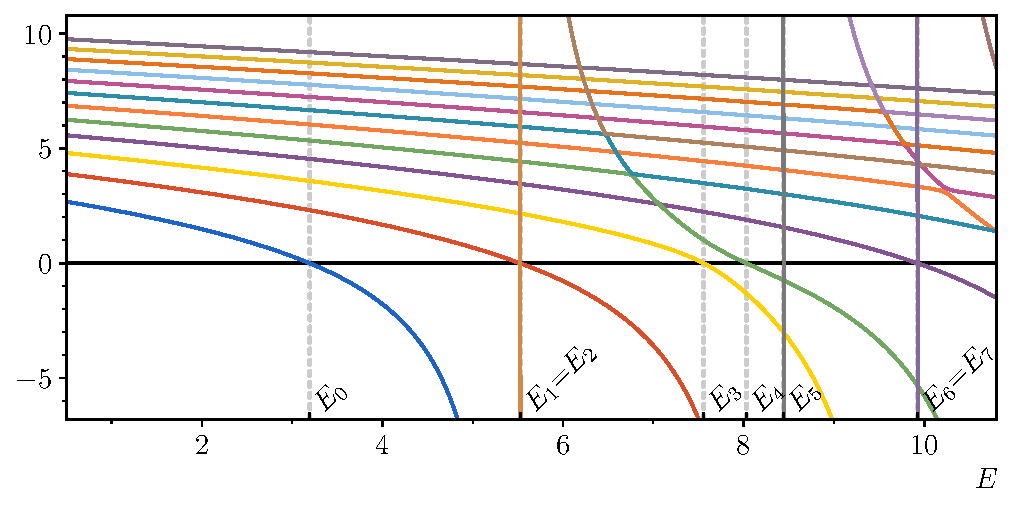
\includegraphics[width=\textwidth]{img/chapter3/mismatch_rainbow.pdf}
  \caption{Each of the eigenvalues $\lambda$ of the mismatch matrix $\vb{\Phi}(E)$ of the Schrödinger problem \eqref{equ:c3_mismatch_ixaru} as a function of $E$. The true eigenvalues of this problem are indicated with $E_0$, $E_1$, $\dots$ The lines are colored and continued to aid in the clarity of this illustration. But, do notice that this is only a best guess approximation.}\label{fig:c3_mismatch_rainbow}
\end{figure}

Throughout this research, one of the first graphs which we studied can be found in figure \ref{fig:c3_mismatch_rainbow}. Here all eigenvalues of the mismatch matrix $\vb{\Phi}(E)$ are plotted. For each value of $E$, in this problem $\vb{\Phi}(E)$ had $N$ real eigenvalues, with $N$ the size of basis on each sector, as described in \ref{sec:c3_ixarus_method}. Upon seeing this graph, it is easy to say, that one can `follow' the trajectory of a single eigenvalue as $E$ changes. In reality, this is not easy at all. For example, sometimes two eigenvalue curves intersect, other times they barely avoid each other, and seemingly switch which curve they follow. In figure \ref{fig:c3_mismatch_rainbow_zoom} this strange behavior is visible. Also note, that following the lowest eigenvalue $\lambda_0$, will  not result in a nice smooth curve, since this value reaches vertical asymptotes.

\begin{figure}
  \begin{center}
    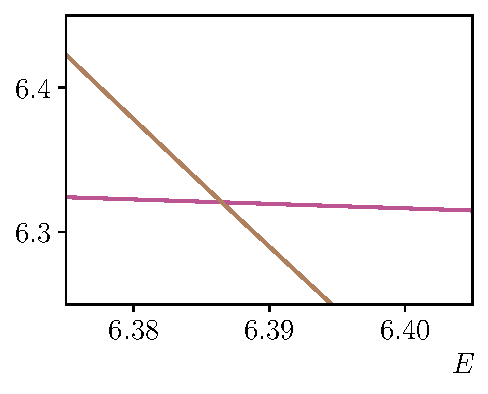
\includegraphics[width=.495\textwidth]{img/chapter3/mismatch_rainbow_zoomed_0.pdf}
    \hfill
    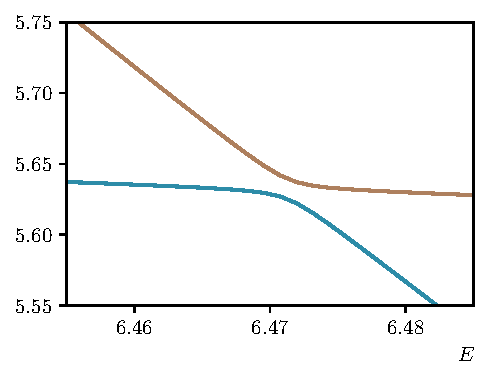
\includegraphics[width=.495\textwidth]{img/chapter3/mismatch_rainbow_zoomed_1.pdf}
  \end{center}
  \caption{These are zoomed in views of the graph from \ref{fig:c3_mismatch_rainbow}. Some surprising behavior of the eigenvalues of $\vb{\Phi}(E)$ are visible.}\label{fig:c3_mismatch_rainbow_zoom}
\end{figure}

These difficulties and nuances are hidden away behind the colors and seemingly continuous lines present in figure \ref{fig:c3_mismatch_rainbow}. Practically, this graph is generated from the eigenvalues (and their derivatives) of $\vb{\Phi}(E)$ for $\numprint{10000}$ values of $E$. Two eigenvalues $\lambda^{(i)}_j$, $\lambda^{(i+1)}_k$  for two adjacent values $E_{i}$ and $E_{i+1}$, are determined to correspond to the same curve (and thus get the same color) if
$$ \lambda^{(i)}_j \approx \lambda^{(i+1)}_k - (E_{i+1} - E_i) \dv[]{\lambda^{(i+1)}_k}{E} $$
is sufficiently accurate.

\begin{figure}
  \centering
  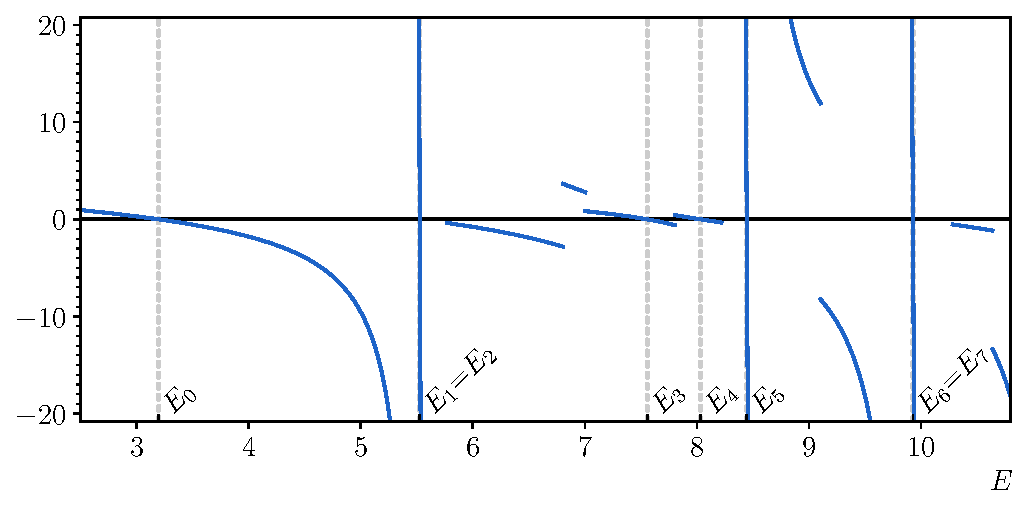
\includegraphics[width=\textwidth]{img/chapter3/mismatch_newton.pdf}
  \caption{The function \eqref{equ:c3_mismatch_newton_function}, derived from problem \eqref{equ:c3_mismatch_ixaru}, is plotted. Notice that this graph can also be found as a part of figure \ref{fig:c3_mismatch_rainbow}. At first glance, the striking vertical lines may be assumed to be asymptotes. This is not the case, in these regions $f(E)$ changes very rapidly.}\label{fig:c3_mismatch_newton}
\end{figure}

In figure \ref{fig:c3_mismatch_newton} the graph of the function $f(E)$ from equation \eqref{equ:c3_mismatch_newton_function} is plotted. Comparing this with figure \ref{fig:c3_mismatch_rainbow}, allows us to get an intuitive understanding of our application of Newton's method. But as can be seen in figure \ref{fig:c3_mismatch_newton}, this method is not perfect. For example, the region in which eigenvalue $E_5$ can be detected is relatively small. If the more straightforward $f(x) = \argmin_{\lambda \in \eigs(\vb{\Phi(E)}) \cap \RR} \left|\lambda\right|$ was used, this region would be even smaller. But still, numerically it would be very unlikely to stumble upon this region, to detect that an eigenvalue was missing. For this reason we have developed a robust way to determine the number of an eigenvalue less than the value $E$. This allows us to detect these missing values, and locate them. In the next section (\ref{sec:c3_index_of_e}), we will develop some new theory to locate all eigenvalues reliably.

\section{Determining the index of eigenvalues}\label{sec:c3_index_of_e}

This section is based upon yet unpublished work, in collaboration with professor Hans Vernaeve.

Throughout mathematical physics there are many problems dependent on, or consisting of determining eigenvalues of a linear elliptic operator on a given domain with homogeneous Dirichlet boundary conditions. Some examples are the Schrödinger equation, the wave equation, the linear theory of elasticity..., to name a few. There are many methods, analytical as well as numerical, to solve for or to approximate these eigenvalues, e.g. shooting methods\cite{ixaru_numerical_1984,ixaru_new_2010}, finite difference methods\cite{wang_new_2009}, methods for finding the lowest eigenvalues\cite{braun_efficient_1996}, or even the methods discussed in chapters \ref{cha:c2}, \ref{cha:c3} and \ref{cha:c4}, \dots There even exist (numerical) methods that are able to find eigenvalues in the neighborhood of a given value $E$ without the need to compute all lower eigenvalues. For this last group of methods we have developed a theorem to count eigenvalues.

\begin{table}
  \newlength{\hoWidth}
  \setlength{\hoWidth}{.2\linewidth}
  \begin{center}
    \begin{tabular}{rlrl|rl|}
      \multicolumn{2}{|c}{$ \lambda_{0} \approx 2.00$}                                                                     & \multicolumn{2}{|c|}{$ \lambda_{1,2} \approx 4.00 $} & \multicolumn{2}{c|}{$ \lambda_{3,4,5} \approx 6.00 $}                                                                                                                                                                                                                                                             \\ \hline
      \multicolumn{1}{|c}{\parbox[c]{\hoWidth}{
\includegraphics[width=\linewidth]{img/chapter3/counting/harmonic/2a.png}}} & $ \begin{matrix} \mathbf{u_{1,1}} \vspace{5pt}\\ \scalebox{1.5}{$\mathbf{1}$} \end{matrix} $                       & \multicolumn{1}{|c}{\parbox[c]{\hoWidth}{
\includegraphics[width=\linewidth]{img/chapter3/counting/harmonic/4a.png}}} & $ \begin{matrix} \mathbf{u_{1,2}} \vspace{5pt}\\ \scalebox{1.5}{$\mathbf{2}$} \end{matrix} $ & \parbox[c]{\hoWidth}{\vspace{2pt}
\includegraphics[width=\linewidth]{img/chapter3/counting/harmonic/6a.png}\vspace{2pt}} & $ \begin{matrix} \mathbf{u_{2,2}} \vspace{5pt}\\ \scalebox{1.5}{$\mathbf{4}$} \end{matrix} $  \\
      \cline{1-6}                                                                                                          &                                                      & \multicolumn{1}{|c}{\parbox[c]{\hoWidth}{
\includegraphics[width=\linewidth]{img/chapter3/counting/harmonic/4b.png}}} & $ \begin{matrix} \mathbf{u_{2,1}} \vspace{5pt}\\ \scalebox{1.5}{$\mathbf{2}$} \end{matrix} $ & \parbox[c]{\hoWidth}{\vspace{2pt}
\includegraphics[width=\linewidth]{img/chapter3/counting/harmonic/6b.png}\vspace{2pt}} & $  \begin{matrix} u_{1,3} \vspace{5pt}\\ \scalebox{1.5}{$3$} \end{matrix} $ \\
      \cline{3-6}                                                                                                          &                                                      &                                                                                                                      &                                & \parbox[c]{\hoWidth}{\vspace{2pt}
\includegraphics[width=\linewidth]{img/chapter3/counting/harmonic/6c.png}\vspace{2pt}} & $ \begin{matrix} u_{3,1} \vspace{5pt}\\ \scalebox{1.5}{$3$} \end{matrix} $  \\
      \cline{5-6}
    \end{tabular}
    \caption{\label{tab:courant_harmonic}Density plots (see also figure \ref{fig:harmonic_3d}) of the first six eigenfunctions of the quantum harmonic oscillator, $-\nabla^2 u + (x^2+y^2) u = \lambda u$, on the square $[-5;5]\times [-5;5]$, with homogeneous Dirichlet boundary conditions. For each eigenfunction the number of nodal domains is indicated. The eigenfunctions for which Courant's nodal domain theorem is strict, are highlighted in bold. These four eigenfunctions presented here are the only ones, for the harmonic oscillator, for which this strictness holds. }
  \end{center}
\end{table}

Up until now there was no method, that the authors know of, to reliably determine the exact number of eigenvalues lower than a given value $E$ for multidimensional problems. The best known result is already almost a century old: Courant's nodal domain theorem \cite[Vol I, Chapter  VI, paragraph 2, Theorem 2]{courant_methods_2008}. This theorem states that for an eigenfunction $u$ with corresponding eigenvalue $\lambda$, there are at least as many eigenvalues, counted with multiplicity, less than $\lambda$ as the number of nodal domains of $u$ minus one \cite[Theorem 1.1]{berard_nodal_2014}. A nodal domain is defined as a largest connected set of the domain on which the eigenfunction $u$ does not become zero. The nodal domain theorem gives, when an eigenvalue $\lambda$ with corresponding eigenfunction is known, a lower bound on the number of eigenvalues less than $\lambda$. However, only for restricted classes of one dimensional problems, this value is exact. In table \ref{tab:courant_harmonic} this fact is demonstrated by showing that the number of nodal domains of an eigenfunction does not lead to an exact estimate for the index of the corresponding eigenvalue.
% Fun fact: Richard Courant maried the daughter of Carl Runge

\begin{figure}
  \begin{center}
    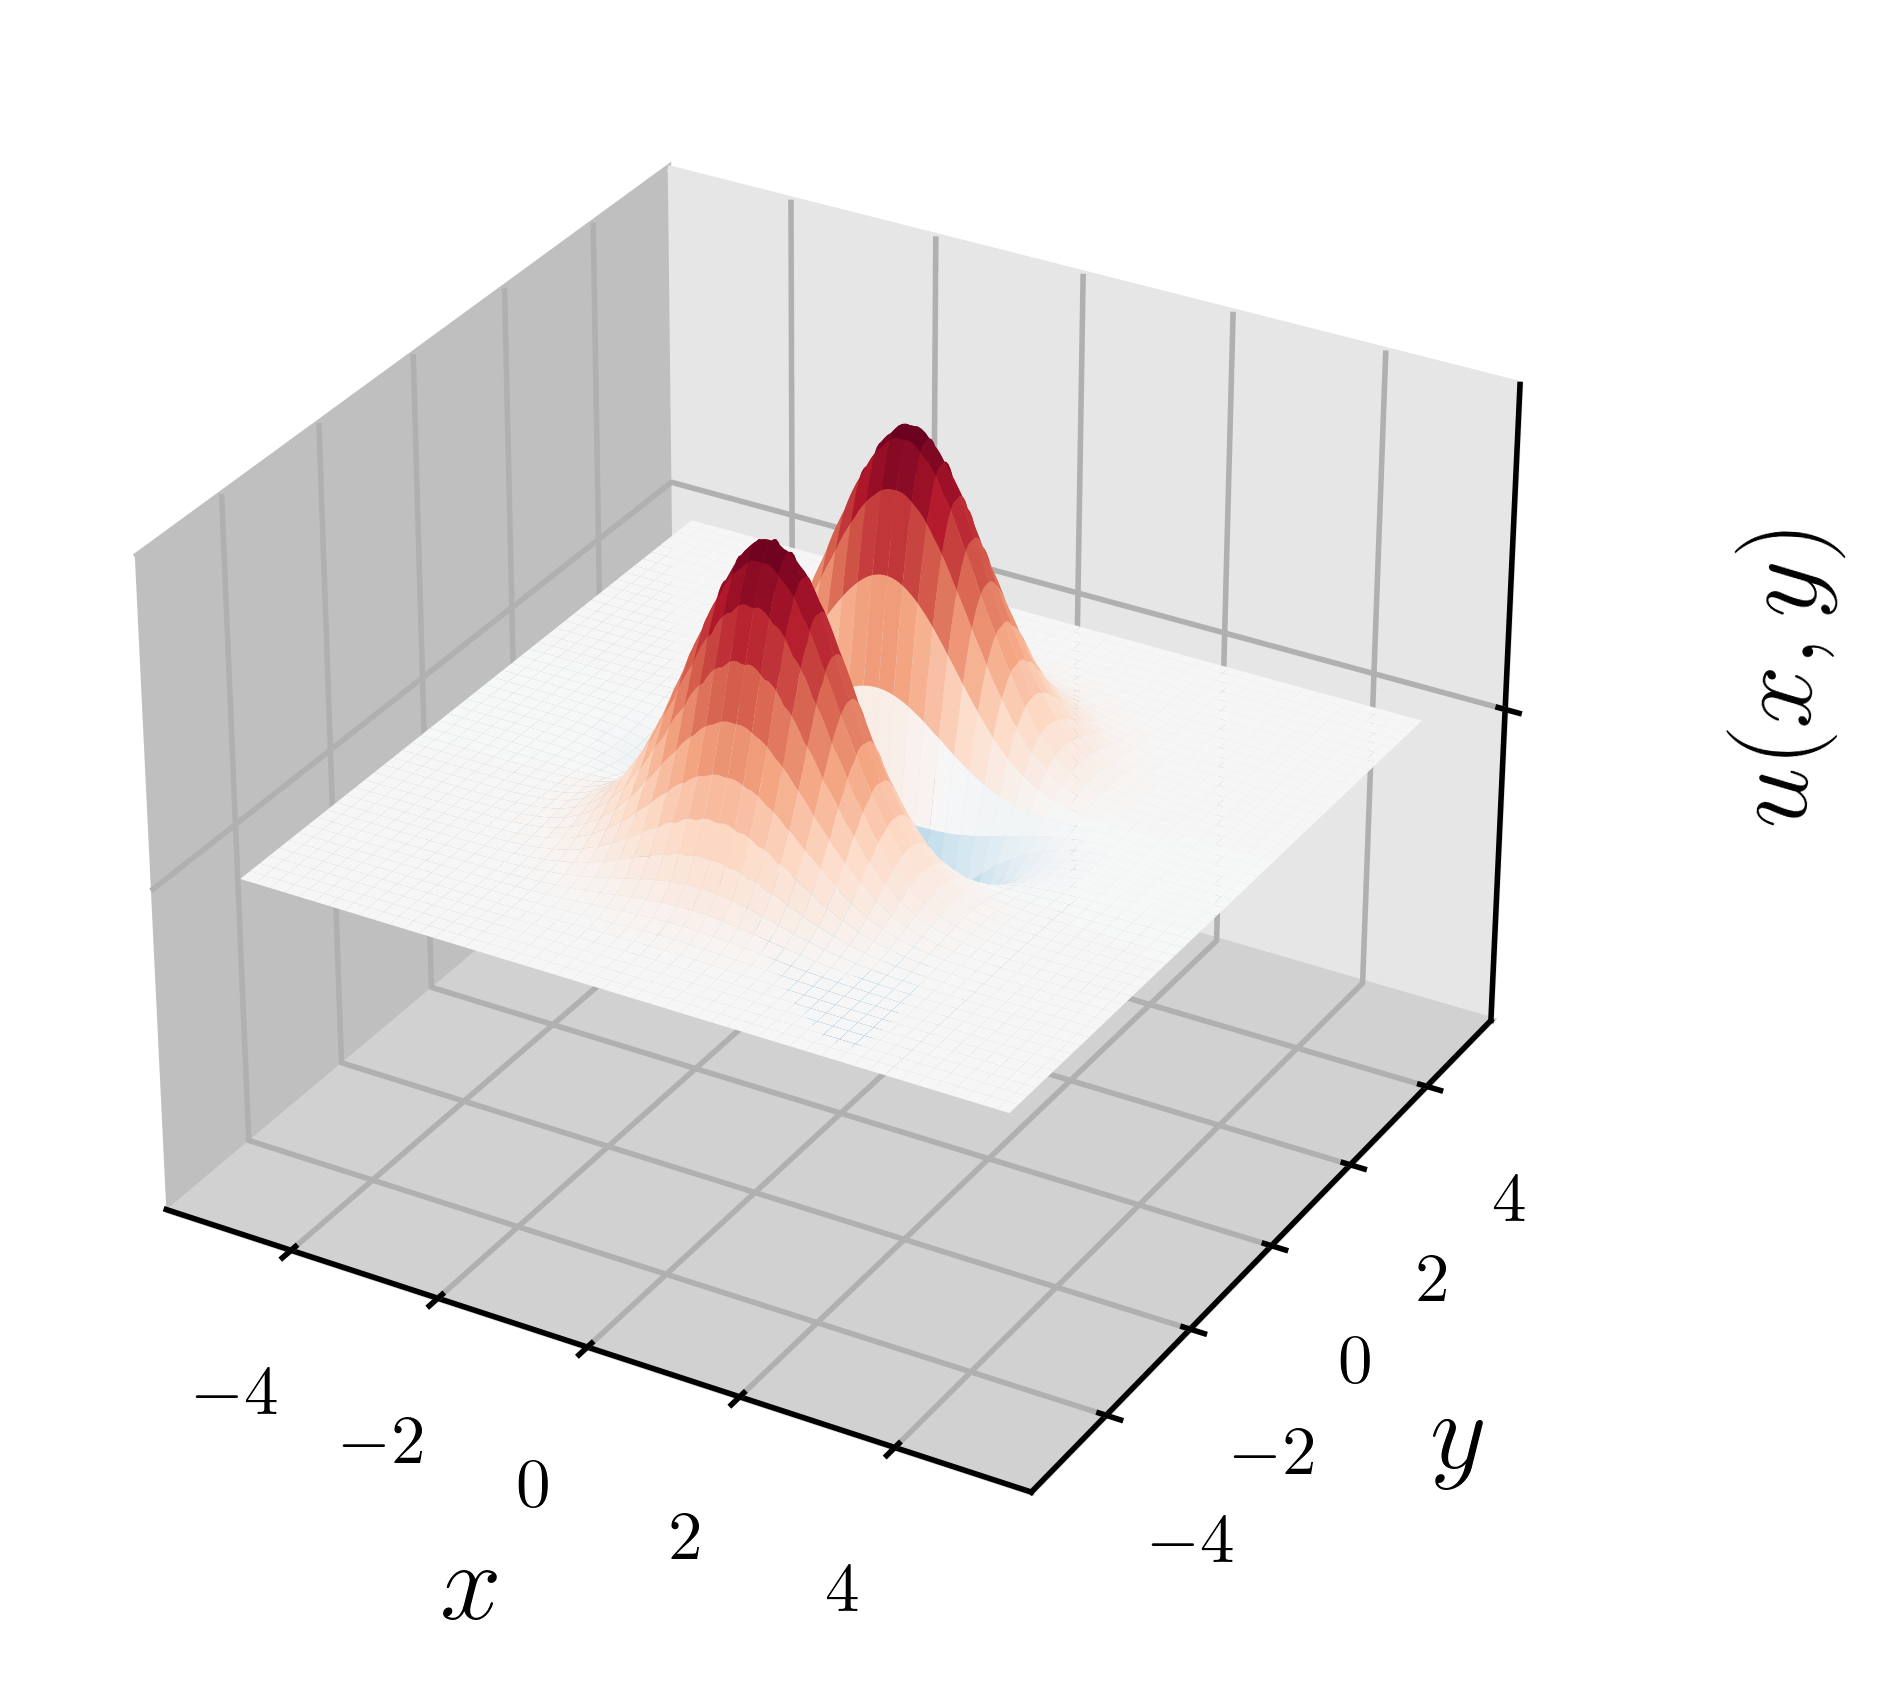
\includegraphics[width=\linewidth]{img/chapter3/counting/harmonic_3d.png}
    \caption{\label{fig:harmonic_3d} A three-dimensional graph of the eigenfunction $u_{3,1}$ of the quantum harmonic oscillator, $-\nabla^2 u + (x^2+y^2) u = \lambda u$, on the square $[-5; 5] \times [-5; 5]$, with homogeneous Dirichlet boundary conditions. This graph illustrates how the density plots from table \ref{tab:courant_harmonic} and figure \ref{fig:c3_disc_solutions} should be interpreted.}
  \end{center}
\end{figure}

A practical problem in applying Courant's nodal domain theorem is that it is, numerically, quite difficult to reliably determine the number of nodal domains of a function. This history and our need to determine the number of eigenvalues less than a certain value $E$ have motivated us to formulate theorem \ref{lem:c3_eigenvalues_curves}.

To develop the necessary theory for this theorem, some definitions are needed. These will simplify the notation and proof of our results.
\begin{definition}
  The one-dimensional cross-section $l_{\Omega,i}(\vb{x})$ of a Lipschitz domain $\Omega$ along the $i^\text{th}$ dimension through $\vb{x}$ is defined as:
  $$
    l_{\Omega,i}(\vb{x}) := \left\{\vb{y} \in \Omega \ |\  \forall j \neq i : \vb{x}_j = \vb{y}_j   \right\}\text{.}
  $$
\end{definition}

Note that, when $\Omega$ is bounded, $l_{\Omega,i}(\vb{x})$ is the union of collinear line segments. As such, the following definition represents the maximal sum of the lengths of each of these segments.

\begin{definition}
  The \emph{directional diameter}, $\dirdiam_i(\Omega)$, of a bounded Lipschitz domain $\Omega \subseteq \RR^n$ is defined as:
  $$
    \dirdiam_i(\Omega) := \sup_{\vb{x}\in\Omega} \int_{-\infty}^{\infty} I_\Omega(\vb{x}_1, \dots, \vb{x}_{i-1}, t, \vb{x}_{i+1}, \dots, \vb{x}_n) \, \dd t \text{.}
  $$
  Here $I_\Omega(\vb{x})$ is defined as $1$ if $\vb{x} \in \Omega$, zero otherwise.
\end{definition}

In theorem \ref{the:c3_counting_eigenvalues} we will be able to identify each eigenvalue by using a continuous sequence of domains $\Omega_\epsilon$. For this sequence of domains it should hold that if $\epsilon \to 0$, the domains should become unboundedly small. The notion of the \emph{directional diameter} allows us to quantify this.

\begin{figure}[t]
  \begin{center}
    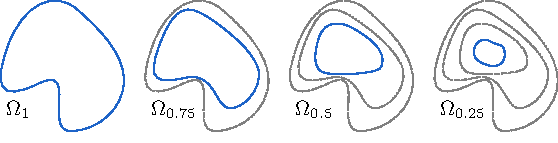
\includegraphics[width=\linewidth]{img/chapter3/counting/main-theorem-omega.pdf}
    \caption{\label{fig:intuitive_example_omega} An example of a sequence of domains $\Omega_\epsilon$ that satisfy the necessary conditions for theorem \ref{the:c3_counting_eigenvalues}: the domains are nested, all domains are Lipschitz, and the horizontal as well as the vertical directional diameter converge to zero for $\epsilon \to 0^{+}$.}
  \end{center}

  \begin{center}
    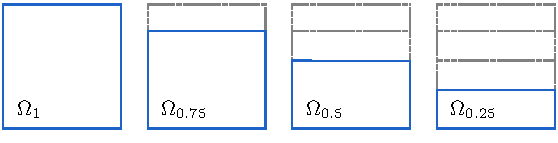
\includegraphics[width=\linewidth]{img/chapter3/counting/main-theorem-rho.pdf}
    \caption{\label{fig:intuitive_example_rho} Another example of a sequence of domains $\Omega_\epsilon$ that also satisfy the necessary conditions for theorem \ref{the:c3_counting_eigenvalues}. Note that these conditions only require that any directional diameter converges to zero. In this example the horizontal directional diameter does not converge to zero: $\lim_{\epsilon \to 0^+}\dirdiam_1(\Omega_\epsilon) \neq 0$. The vertical directional diameter does vanish: $\lim_{\epsilon \to 0^+}\dirdiam_2(\Omega_\epsilon) = 0$.}
  \end{center}
\end{figure}

In figures \ref{fig:intuitive_example_omega} and \ref{fig:intuitive_example_rho}, two examples of series of domains are given. Both of these sets of domains are applicable for theorem \ref{the:c3_counting_eigenvalues}. We would like to note that the domain from figure \ref{fig:intuitive_example_rho} is particularly valuable for \cite{ixaru_new_2010} and our work\cite{baeyens_improvements_2022} in this chapter.



The next section will be dedicated to proving this theorem. In the last section we will provide some examples of and motivation for our work.


\subsection{The main theorem} \label{sec:main_theorem}

Throughout this section the $L^2$-norm $\|\cdot\|_{L^2(\Omega)}$ and Sobolev norm $\|\cdot\|_{H^k(\Omega)}$ are being used. For clarity, we will provide the necessary definitions. For a more thorough discussion of these norms and their properties many texts are available, for example \cite{adams_sobolev_2003}.

Let $L^2(\Omega)$ be the space of functions $u : \Omega \to \RR$ such the norm
$$
  \|u\|_{L^2(\Omega)} := \left(\int_\Omega \left| u \right|^2 \right)^{\frac{1}{2}}
$$
exists and is finite.

The Sobolev space $ H^k(\Omega) = W^{k, 2}(\Omega) $ is the space of all functions $u \in L^2(\Omega)$ such that, for the multi-index $\alpha$ with order $|\alpha|$ at most $k$, each weak partial derivative $D^\alpha u$ of $u$ is a function in $L^2(\Omega)$. The Sobolev norm of $u$ is defined as:
$$
  \|u\|_{H^k(\Omega)} := \left(\sum_{|\alpha| \leq k} \int_\Omega \left| D^\alpha u \right|^2\right)^{\frac{1}{2}}\text{.}
$$

The subspace $ H^k_0(\Omega)$ of $H^k(\Omega)$ is the closure of all infinitely differentiable compactly supported functions on $\Omega$ in $H^k(\Omega)$.

Before proving the main theorem of this article we provide a kind of Fried\-richs's inequality to estimate a lower bound for $\| u \|_{H^k(\Omega)}$ in terms of $\| u \|_{L^2(\Omega)}$, and the diameter and any directional diameter of $\Omega$.

\begin{lemma}
  \label{lem:friederichs_like}
  Let $\Omega \subset \RR^n$ be a bounded domain with Lipschitz boundary, and $k \in \mathbb{N}^{+}$. For each $u \in H_0^k(\Omega)$, and any $j \leq n$
  \begin{equation}
    \label{equ:friederichs_like}
    \| u \|_{L^2(\Omega)} \leq \sqrt{\diam(\Omega) \dirdiam_j(\Omega)} \| u \|_{H^k(\Omega)} \text{.}
  \end{equation}
\end{lemma}
\begin{proof}
  For ease of notation, we will assume $j = 1$. Note that this proof is equally valid for any other $j$. Assume also $u \in C^\infty_c(\Omega) \cap H_0^k(\Omega)$. Because of the homogeneous Dirichlet boundary conditions,
  the fundamental theorem of calculus can be used to estimate $|u(\vb{x})|^2$ for each $\vb{x} \in \Omega$
  $$
    \left|u(\vb{x})\right|^2 = \left|\int_{-\infty}^{\vb{x}_1} \pdv[]{u}{x_1}\left(t, \vb{x}_2, \dots, \vb{x}_{n}\right)I_\Omega(t,\vb{x}_2, \dots, \vb{x}_n)\dd t\right|^2 \text{.}
  $$
  In this formula, and throughout the proof, we formally pose that $u(\vb{x}) \equiv 0$ for $\vb{x} \notin \Omega$. Note that the fundamental theorem of calculus is applicable because $u$ is compactly supported and in $C^1$.

  Applying the Cauchy-Schwarz inequality provides some simplifications. Growing the integration domain removes the dependency on $\vb{x}_1$.
  \begin{align*}
    \left|u(\vb{x})\right|^2 & \leq \int_{-\infty}^{\vb{x}_1} I_\Omega(t,\vb{x}_2, \dots, \vb{x}_n) \dd t \int_{-\infty}^{\vb{x}_1} \left|\pdv[]{u}{x_1}\left(t,\vb{x}_2, \dots, \vb{x}_n\right)\right|^2\dd t \\
                             & \leq \dirdiam_1(\Omega) \int_{a}^{b} \left|\pdv[]{u}{x_1}\left(t,\vb{x}_2, \dots, \vb{x}_n\right)\right|^2\dd t
  \end{align*}
  with $a = \inf_{\vb{x} \in \Omega}\{\vb{u}_1 \,|\, \forall \vb{u} \in l_{\Omega, 1}(\vb{x})\}$ and $b = \sup_{\vb{x} \in \Omega}\{\vb{u}_1 \,|\, \forall \vb{u} \in l_{\Omega, 1}(\vb{x})\}$. Integrating both sides over $\Omega$, applying Fubini's theorem, and noting that $b - a \leq \diam(\Omega)$, yields the required expression for $u \in C^\infty_c(\Omega)$.
  \begin{align*}
    \|u\|_{L^2(\Omega)}^2 & \leq \dirdiam_1(\Omega) \int_\Omega \int_{a}^{b} \left|\pdv[]{u}{x_1}\left(t, \vb{x}_2, \dots, \vb{x}_{n}\right)\right|^2\dd t \, \dd \vb{x} \\
                          & = \dirdiam_1(\Omega) \, (b - a) \, \int_{\Omega} \left|\pdv[]{u}{x_1}\left(\vb{x}\right)\right|^2 \dd \vb{x}                                 \\
                          & \leq \dirdiam_1(\Omega) \, \diam(\Omega) \, \| u \|^2_{H^k(\Omega)}
  \end{align*}

  To prove this for each $u \in H_0^k(\Omega)$, we only have to note that
  $C^\infty_0(\Omega)$ is $H^k(\Omega)$-dense in $H^k_0(\Omega)$. Now $u \in H_0^k(\Omega)$ can be written as $u = \lim_{i \to +\infty} u_i$ with $u_i \in C^\infty_c(\Omega)$. This implies that
  $$\|u\|_{L^2(\Omega)}^2 \leq \dirdiam_1(\Omega) \, \diam(\Omega) \, \| u \|^2_{H^k(\Omega)}\text{,}$$
  for each $u \in H_0^k(\Omega)$.
\end{proof}

Now we are able to prove lemma \ref{lem:c3_eigenvalues_curves}. This prepares the main result of this section: theorem \ref{the:c3_counting_eigenvalues}.

\begin{lemma}\label{lem:c3_eigenvalues_curves}
  Let $\left\{\Omega_\epsilon \subseteq \RR^n \ | \ \forall \epsilon \in \left]0, 1\right]\right\}$ be a continuous family of diffeomorphic bounded Lipschitz domains, such that $ a < b \implies \Omega_a \subsetneq \Omega_b $, and
  $$
    \exists j : \lim_{\epsilon \to 0^{+}} \dirdiam_j(\Omega_\epsilon) = 0\text{.}
  $$

  Let $\mathcal{L}$ be a linear self-adjoint uniformly elliptic operator, defined on $\Omega_1$. Define $\lambda_{\epsilon,i}$ as the $i^\text{th}$ eigenvalue of $\mathcal{L}$ limited to $\Omega_\epsilon$ with homogeneous Dirichlet boundary conditions. Then for each $i \in \mathbb{N}$, the values $\lambda_{\epsilon,i}$ as functions of $\epsilon$
  \begin{itemize}
    \item are continuous,
    \item are strictly decreasing,
    \item and are unbounded for $\epsilon \to 0^{+}$.
  \end{itemize}
\end{lemma}
\begin{proof}
  Already in 1924 Courant and Hilbert \cite[Vol I. Chapter V. Paragraph 13]{courant_methods_2008} noted the continuity of the spectrum given perturbations of the elliptic operator. Hale described (e.g.\ \cite{hale_eigenvalues_2005}) how to translate regular perturbations in the domain to perturbations in the operator. Our set of diffeomorphic domains satisfies the necessary assumptions formulated by Hale, so continuity is guaranteed.

  That $\lambda_{\epsilon, i}$ is a decreasing function of $\epsilon$, can be shown by application of \cite[Vol I, Chapter  VI, paragraph 2, Theorem 3]{courant_methods_2008} \emph{``Under the boundary condition $u = 0$ the $n^\text{th}$ eigenvalue for a domain $G$ never exceeds the $n^\text{th}$ eigenvalue for a subdomain of $G$".} The strictness is addressed in a footnote by this theorem: \emph{"In fact, it is always smaller when we are dealing with a proper subdomain."}.

  To prove that $\lambda_{\epsilon, i}$ grows unboundedly we start with Gårding's inequality \cite[Section 9.2.3]{renardy_introduction_2004}. It says that there exist $C_1$ and $C_2$ such that for all $u \in H^k_0(\Omega_\epsilon)$:
  \begin{equation}\label{equ:garding}
    \frac{\bra{\mathcal{L}u}\ket{u}_{L^2(\Omega_\epsilon)}}{\|u\|_{L^2(\Omega_\epsilon)}^2} + C_1 \geq C_2 \frac{\|u\|_{H^k(\Omega_\epsilon)}^2}{\|u\|_{L^2(\Omega_\epsilon)}^2}
  \end{equation}
  Note that the same $C_1$ and $C_2$ as for $\Omega_1$ will also work for $\Omega_\epsilon$. Lemma \ref{lem:friederichs_like} provides an estimate for the right-hand side of \eqref{equ:garding}, which, in turn, provides an estimate for the operator $\mathcal{L}$:
  $$
    \frac{\bra{\mathcal{L}u}\ket{u}_{L^2(\Omega_\epsilon)}}{\|u\|_{L^2(\Omega_\epsilon)}^2} \geq \frac{C_3}{\sqrt{\dirdiam_j(\Omega_\epsilon)}} - C_1\text{,}
  $$
  for a constant $C_3$. By assumption the right-hand side is unbounded for $\epsilon \to 0$. Substituting the eigenfunction $u_{\epsilon, i}$ corresponding to the eigenvalue $\lambda_{\epsilon, i}$ into the left-hand side, yields that $\lambda_{\epsilon, i}$ has to be unbounded as well.
\end{proof}

\begin{figure}
  \begin{center}
    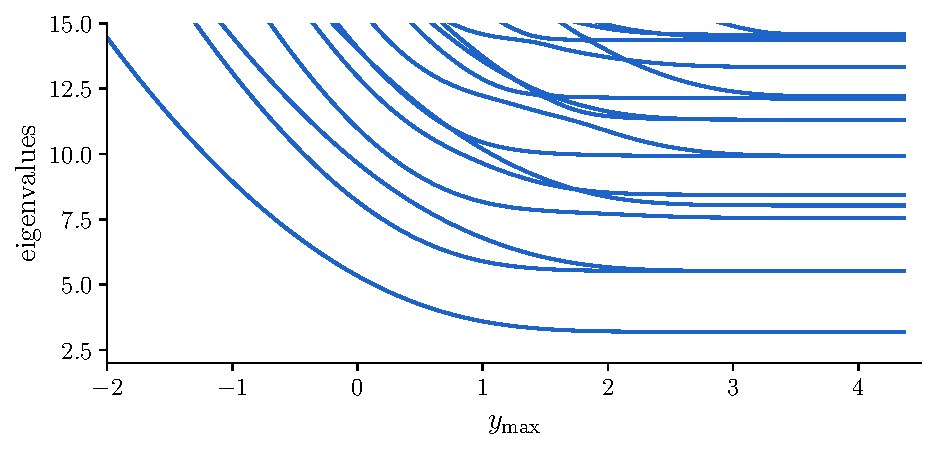
\includegraphics[width=\textwidth]{img/chapter3/counting/counting_eigenvalues.pdf}
    \caption{This graph displays all eigenvalues less than $15$ for the two-dimensional Schrödinger problems $-\nabla^2 \psi + (1+x^2)(1+y^2)\psi = E \psi$ on the rectangle $[-5.5; 5.5]\times[-5.5; y_{\text{max}}]$ with homogeneous Dirichlet boundary conditions.}\label{fig:c3_counting_eigenvalue_graph}
  \end{center}
\end{figure}

As an example, in figure \ref{fig:c3_counting_eigenvalue_graph} the spectrum of a Schrödinger operator is plotted as a function of the nested sequence of domains $[-5.5; 5.5] \times [-5.5; y_{\text{max}}]$. Each curve corresponds to an eigenvalue. The figure suggests that all of these lines are continuous, decreasing, and unbounded for $y_{\text{max}} \to -5.5^{+}$, in accordance with lemma \ref{lem:c3_eigenvalues_curves}. A horizontal line corresponding to a fixed value $E$ will intersect each curve corresponding to a lower eigenvalue on the whole domain. This number of
intersection thus gives the number of eigenvalues lower than this given value $E$. If $E$ itself is an eigenvalue, then we have also found its index.

The graph from figure \ref{fig:c3_counting_eigenvalue_graph} and the notion of a horizontal line with fixed value of $E$, give rise to following theorem.

\begin{theorem}[Baeyens, Van Daele and Vernaeve 2022]\label{the:c3_counting_eigenvalues}
  Let $\mathcal{L}$ be a linear self-adjoint uniformly elliptic operator on a bounded Lipschitz domain $\Omega_1 \subseteq \RR^n$ with homogeneous Dirichlet boundary conditions. Define, following \cite{hale_eigenvalues_2005}, a topology on all domains $\Omega$ which are $C^k$-diffeomorphic to $\Omega_1$.  Assume a continuous family of such $C^k$-diffeomorphic domains $\Omega_\epsilon$ for $\epsilon\in\left]0; 1\right]$ is given such that $\Omega_a \subseteq \Omega_b$ if $a < b$ and $\exists j : \lim_{\epsilon\to 0^+} \dirdiam_j(\Omega_\epsilon) = 0$.

  For a given value $E$ the number of eigenvalues of $\mathcal{L}$ on $\Omega_1$ less than or equal to $E$ is exactly the same as the number of domains $\Omega_\epsilon$ on which $E$ is an eigenvalue of $\mathcal{L}$ limited to $\Omega_\epsilon$ with homogeneous Dirichlet boundary conditions. Domains on which $E$ is an eigenvalue with multiplicity $d$ are counted $d$ times.
\end{theorem}

As a necessary condition we imposed that, for the sequence of domains $\Omega_\epsilon$,
$$
  \dirdiam_j(\Omega_\epsilon)
$$
should converge to zero. This may seem a quite restrictive condition, in practice it is not. Most, natural, sequences of domains do satisfy this condition in at least one axis. In the next section we provide some examples of different kinds of such domains.

For direct methods, such as (semi-)discretization methods, theorem \ref{the:c3_counting_eigenvalues} cannot directly be applied. However, for shooting methods (\cite{ixaru_new_2010,baeyens_improvements_2022}) this theorem is extremely useful.
In such methods, for a fixed value of $E$, an error function is computed by propagating solutions over the domain. The error function measures the mismatch between the propagated solution and the boundary conditions.

While propagating a solution one can keep track of how many times the boundary conditions are met inside the domain. Each of these occurrences corresponds to a subdomain on which $E$ is an eigenvalue, which in turn, by theorem \ref{the:c3_counting_eigenvalues}, corresponds to a unique eigenvalue less than $E$.


\subsection{Examples}\label{sec:c3_counting_examples}

We provide a few examples. The first example illustrates that our result is a more general formulation for a well known theorem for the one-dimensional problem. In the second example we will do some symbolic calculations for a disc-shaped domain. The third example will demonstrate our implemention of theorem \ref{the:c3_counting_eigenvalues} in the method from section \ref{sec:c3_ixarus_method}. And in the last example we will take a look at a much more exotic family of domains to illustrate the applicability of our theorem to use-cases far beyond what our numerical method is capable of.

\subsubsection{One dimensional Sturm-Liouville equation}

Let $\lambda_i$ be the $i^{\text{th}}$ eigenvalue\footnote{The first eigenvalue is denoted as $\lambda_0$, the second as $\lambda_1$\dots}, with eigenfunction $y_i(x)$, of the Sturm-Liouville equation
$$
  -\dv{x} \left( p(x) \dv{y_i}{x} \right) + q(x) y_i = \lambda_i w(x) y_i
$$
on the interval $[a, b]$ with homogeneous Dirichlet boundary conditions $y_i(a) = y_i(b) = 0$. Defining the series of domains $\Omega_\epsilon = [a, a + \epsilon\,(b-a)]$, allows us to apply theorem \ref{the:c3_counting_eigenvalues}. Thus, there should be $i$ intervals $\Omega_{\epsilon_j}$, smaller than $[a, b]$, on which $\lambda_i$ is an eigenvalue. As eigenfunctions are unique, up to a scaling factor, $y_i$ should have exactly $i$ zeros inside $[a, b]$. This is a well-known property in Sturm-Liouville theory, see theorem \ref{the:c2_kth_eigen_k_roots}. This fact is also illustrated in figure \ref{fig:c3_counting_sturm_liouville} for the Bessel equation.

\begin{figure}
  \begin{center}
    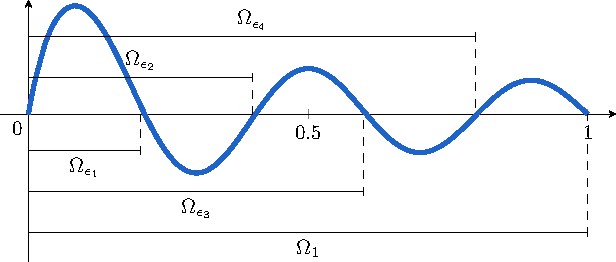
\includegraphics[width=.9\textwidth]{img/chapter3/counting/sturm-liouville.pdf}
    \caption{Eigenfunction $y_4$, with $\lambda_4 \approx 246.74$, of the $\nicefrac{1}{2}$-order Bessel equation\cite{titchmarsh_eigenfunction_1962} $-\dv{x}{} \left( x \dv{y}{x} \right) + \frac{1}{4x} y = \lambda x y $ on $[0, 1]$, with $y(0) = y(1) = 0$. The four subintervals, $\Omega_{\epsilon_1} = [0, \epsilon_1],\dots, \Omega_{\epsilon_4} = [0, \epsilon_4]$, on which $\lambda_4$ is also an eigenvalue of this equation, are indicated.}\label{fig:c3_counting_sturm_liouville}
  \end{center}
\end{figure}

Multiple shooting procedures \cite{baeyens_fast_2020,ledoux_matslise_2016,ixaru_cp_2000} have been developed that implement this using the Prüfer transformation\cite{pruefer_neue_1926}.

\subsubsection{Standing waves on a disc}\label{sec:c3_standing_waves_on_disc}

Consider the eigenvalues and eigenfunctions of the two-dimensional wave equation
\begin{equation}\label{equ:c3_disc_before_polar}
  -\nabla^2 \psi(x, y) = \lambda \psi(x, y)
\end{equation}
on the unit disc with homogeneous Dirichlet boundary condition.

In many introductory textbooks to (partial) differential equations the study of the wave equation on a drum is considered. In most texts, if not all, the idea boils down to: with a transformation to polar coordinates and separation of variables this two-dimensional problem can be transformed into two one-dimensional problems. One of these can be solved directly, the other gives rise to the so-called Bessel functions.

Here we will give a brief overview of the symbolic calculations to solve \eqref{equ:c3_disc_before_polar} on the unit disc $B(\vb{0}, 1)$, with homogeneous Dirichlet boundary conditions. For more details one could consult for example \cite[chapter~4]{asmar_partial_2005}. As stated we first transform \eqref{equ:c3_disc_before_polar} to polar coordinates. For this we pose $x = r\cos(\theta)$ and $y = r\sin(\theta)$, with $r \in [0,1]$ and $\theta \in [0, 2\pi]$. The solutions $u(r, \theta) := \psi(r\cos(\theta), r\sin(\theta))$ are now considered in the transformed domain. Applying the chain rule to $\nabla^2\psi$, yields the new equation
\begin{equation}\label{equ:c3_disc_after_polar}
  -{\pdv[2]{u}{r}} - \frac{1}{r}{\pdv[]{u}{r}} - \frac{1}{r^2} {\pdv[2]{u}{\theta}} = - \lambda u\text{.}
\end{equation}
The boundary conditions are likewise transformed: $u(1, \theta) = 0$ for all $\theta \in [0, 2\pi]$ and $u(r, 0) = u(r, 2\pi)$ and ${\pdv[]{u}{\theta}}(r, 0) = {\pdv[]{u}{\theta}}(r, 2\pi)$ for all $r \in [0, 1]$.

Now we use the method of separation of variables to transform \eqref{equ:c3_disc_after_polar} into two one-dimensional problems. For this, we separate $u(r, \theta) = R(r) \Theta(\theta)$ into a product of an $r$-dependent function and a $\theta$-dependent function. This allows us to write
$$
  -\frac{r^2 R''}{R} - \frac{rR'}{R} - \frac{\Theta''}{\Theta} = \lambda r^2 \text{.}
$$
Rearranging terms to an $r$-dependent side and a $\theta$-dependent side yields two separate equations
\begin{align*}
  \lambda r^2 + \frac{r^2 R''}{R} + \frac{rR'}{R} & = k & \text{and} &  & -\frac{\Theta''}{\Theta} & = k\text{,}
\end{align*}
with $k$ a constant and boundary conditions $R(1) = 0$, $\Theta(0) = \Theta(2\pi)$ and $\Theta'(0) = \Theta'(2\pi)$.

Solutions for $\Theta(\theta)$ can directly be found, as a solution of a linear second order differential equation with constant coefficients. Thus, $\Theta$ only has periodic solutions
$$
  \Theta(\theta) = A_m \cos(m\theta) + B_m \sin(m\theta)\text{,}
$$
if $k = m^2$ with $m \in \{0, 1, 2, \dots\}$. Note that if $m > 0$, there are two linear independent solutions for $\Theta$.

The differential equation for $R(r)$ becomes
$$
  r^2 R'' + r R + (\lambda r^2 - m^2)R = 0\text{.}
$$
We find that solutions to our equation can be written using the $m^\text{th}$ so-called Bessel function of the first kind $R(r) = J_m(r \sqrt{\lambda})$, for more details about these functions see for example \cite[section~4.7]{asmar_partial_2005}. These solutions only satisfy the boundary condition $R(1) = 0$, if and only if $\sqrt{\lambda}$ is a positive zero of $J_m$. If we denote $j_{m, n}$ as the $n^\text{th}$ positive root of the $m^\text{th}$ Bessel function $J_m$ we find that all eigenvalues of \eqref{equ:c3_disc_after_polar} and also of \eqref{equ:c3_disc_before_polar} are given as the squares of roots of the Bessel functions. So $\lambda = j_{m, n}^2$ is an eigenvalue of \eqref{equ:c3_disc_before_polar}. It is single eigenvalue if $m = 0$, otherwise it is a double eigenvalue. The following table contains the first ten eigenvalues, counted with multiplicity.

\begin{center}
  \bgroup
  \def\arraystretch{1.5}
  \begin{tabular}{r|cccccc}
    Eigenvalue       & $\lambda_0$ & $\lambda_{1,2}$ & $\lambda_{3,4}$ & $\lambda_{5}$ & $\lambda_{6,7}$ & $\lambda_{8,9}$ \\ \hline\hline
    Analytical value & $j_{0,1}^2$ & $j_{1,1}^2$     & $j_{2,1}^2$     & $j_{0,2}^2$   & $j_{3,1}^2$     & $j_{1,2}^2$     \\ \hline
    Numerical value  & $5.783$     & $14.68$         & $26.37$         & $30.47$       & $40.71$         & $49.22$
  \end{tabular}
  \egroup
\end{center}

To apply theorem \ref{the:c3_counting_eigenvalues} we need to define a family of domains. A most obvious choice would be all concentric discs with radius at most one. With a variable substitution we know the eigenvalues of the wave equation on $\Omega_\epsilon := B(\vb{0}, \epsilon)$ to be $\frac{\lambda_{i}}{\epsilon^2}$ for all eigenvalues $\lambda_{i}$ on the unit disc. It is obvious that the eigenvalues $\frac{\lambda_{i}}{\epsilon^2}$ as a function of $\epsilon$, are continuous, decreasing, and unbounded as $\epsilon \to 0^{+}$. This confirms lemma \ref{lem:c3_eigenvalues_curves}.

Concentric discs may not be the most thrilling examples. But in the example in section \ref{sec:c3_counting_exotic_domain} we will consider a much more interesting family of domains for the wave equation on a disc.

\subsubsection{A two-dimensional Schrödinger equation}\label{exa:ixaru}

In this example we will take a look at a two-dimensional time-independent Schrödinger equation with homogeneous Dirichlet boundary conditions on a rectangle.
$$
  -\nabla^2 \psi + V(x, y)\psi = E\psi
$$

In section \ref{sec:c3_experiment_ixaru} we will study the Schrödinger problem with the potential
$$
  V(x, y) = (1+x^2)(1+y^2)
$$
on the square $[-5.5; 5.5] \times [-5.5; 5.5]$ with homogeneous Dirichlet boundary conditions. The first eigenvalues are reported in \cite{ixaru_new_2010} to be as follows.

\begin{center}
  \begin{tabular}{r|n{1}{7}cr|n{2}{7}}
    $E_{0}$         & 3.1959181 & \hspace*{2cm} & $E_{6} = E_{7}$ & 9.9280611  \\
    $E_{1} = E_{2}$ & 5.5267439 &               & $E_{8} = E_{9}$ & 11.3118171 \\
    $E_{3}$         & 7.5578033 &               & $E_{10}$        & 12.1032536 \\
    $E_{4}$         & 8.0312723 &               & $E_{11}$        & 12.2011790 \\
    $E_{5}$         & 8.4445814 &               & $E_{12}$        & 13.3323313
  \end{tabular}
\end{center}

\begin{figure}
  \begin{center}
    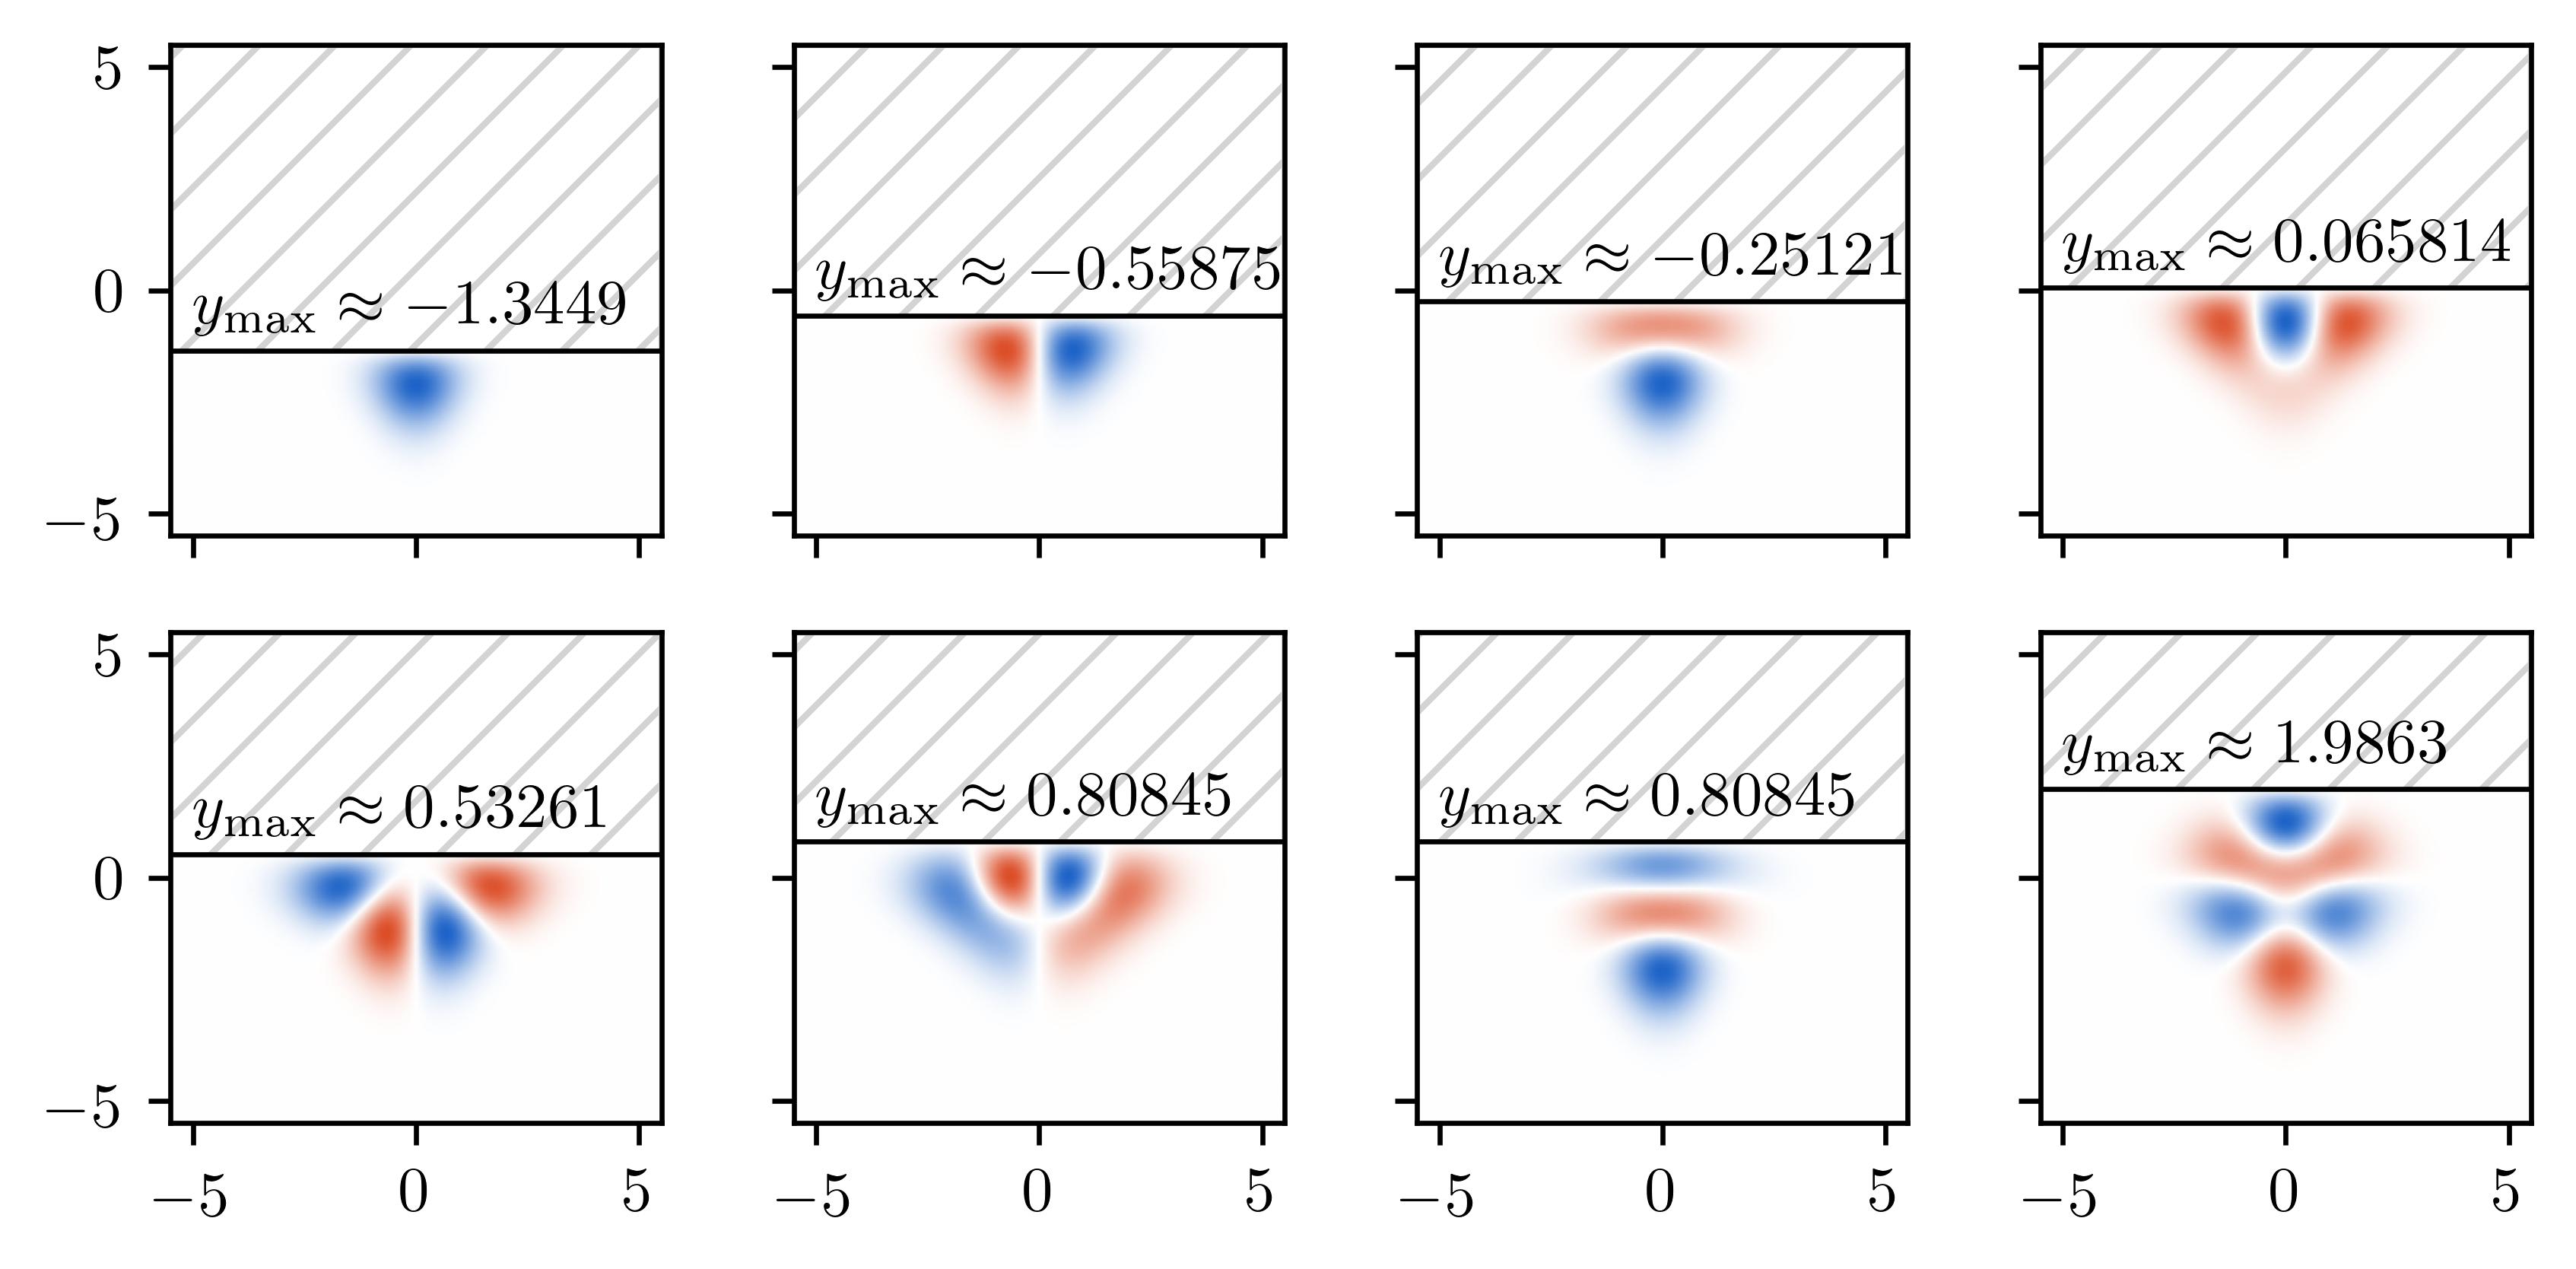
\includegraphics[width=1\textwidth]{img/chapter3/counting/ixaru.png}
    \caption{There are 8 smaller rectangles on which $E = 11$ is an eigenvalue of the Schrödinger equation from example \ref{exa:ixaru}.}\label{fig:c3_counting_ixaru_subdomains}
  \end{center}
\end{figure}

For this problem we will use the method as described in section \ref{sec:c3_ixarus_method}. In summary, this is a shooting method. Which means that it guesses a value for $E$ and calculates a matching error. The matching error in turn is used to improve the estimation of $E$. This process is repeated until $E$ is found up to the desired accuracy.

This matching error is calculated by propagating all possible eigenfunctions $u(x, y)$ from the bottom and the top of the domain to the matching line. In the context of theorem \ref{the:c3_counting_eigenvalues}, this propagation can be thought of as going through all possible subdomains from figure \ref{fig:intuitive_example_rho}. If while propagating, any of the possible eigenfunctions $u$ becomes identically zero on a line, then a subdomain is found on which $E$ is an eigenvalue.

For each $E$, while propagating, one can keep track of how many $u$ did become zero on a line, or in other words, on how many subdomains $E$ is an eigenvalue. Following theorem \ref{the:c3_counting_eigenvalues}, this number tells us how many eigenvalues there are less than $E$ on the whole domain. In figure \ref{fig:c3_counting_ixaru_subdomains}, keeping track of when an eigenfunction becomes zero on a line is demonstrated. For $E = 11$ all domains are visualized where any $u(x, y) = 0$ for all $x \in [\xmin, \xmin]$. Notice that there may be domains on which multiple eigenfunctions are found for that particular value of $E$. These domains should be counted as many times. In figure \ref{fig:c3_counting_ixaru_subdomains}, we see that $\ymax \approx \numprint{0.80845}$ is counted twice. From the tabulated true eigenvalues in \cite{ixaru_new_2010}, we know that there are indeed exactly $8$ eigenvalues less than $E = 11$. This example thus verifies theorem \ref{the:c3_counting_eigenvalues} as well.

\begin{figure}
  \begin{center}
    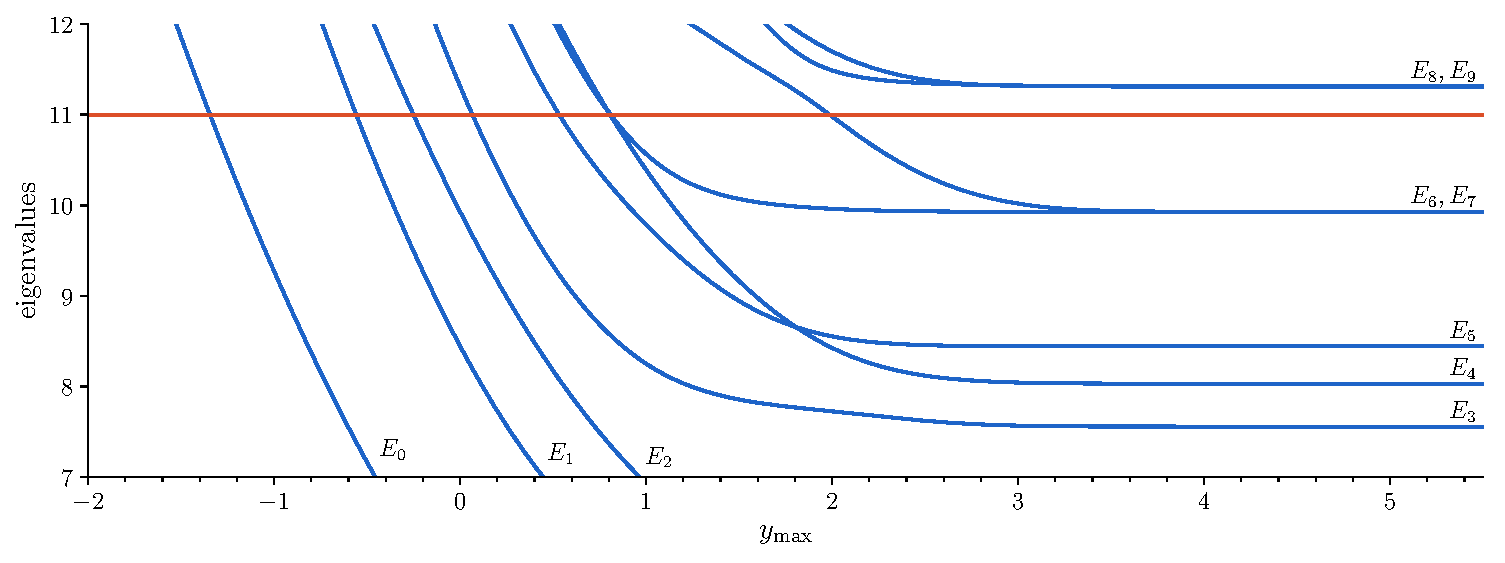
\includegraphics[width=1\textwidth]{img/chapter3/counting/counting_eigenvalues_zoom.pdf}
    \caption{Here a zoomed in version of figure \ref{fig:c3_counting_eigenvalue_graph} is displayed. Each blue graph represents an eigenvalue of the Schrödinger equation from example \ref{exa:ixaru}. The fixed line $E = 11$ is represented in red. Each crossing of the red line and a blue graph represents a smaller subdomain on which $E=11$ is an eigenvalue. These subdomains, with corresponding eigenfunction are illustrated in figure \ref{fig:c3_counting_ixaru_subdomains}.}\label{fig:counting_eigenvalues_zoom}
  \end{center}
\end{figure}

For completeness, we will also verify lemma \ref{lem:c3_eigenvalues_curves} by taking a closer look at the graph from figure \ref{fig:c3_counting_eigenvalue_graph}. In figure \ref{fig:counting_eigenvalues_zoom} we see a zoomed version. These graphs describe how the eigenvalues evolve through the growing domain. If we draw a horizontal line at $E = 11$, as in figure \ref{fig:counting_eigenvalues_zoom}, $8$ curves intersect this line. Each curve corresponds to a lower lying eigenvalue, just like lemma \ref{lem:c3_eigenvalues_curves} predicts.


\subsubsection{A more exotic family of domains}\label{sec:c3_counting_exotic_domain}

\begin{figure}
  \begin{center}
    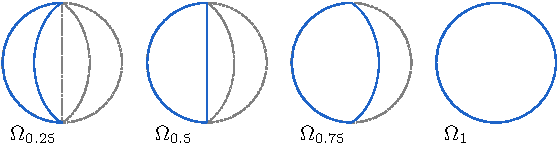
\includegraphics[width=\linewidth]{img/chapter3/counting/moons.pdf}
    \caption{An illustration of the family of domains we consider in section \ref{sec:c3_counting_exotic_domain}.}\label{fig:c3_counting_visual_moons}
  \end{center}
\end{figure}

As a numerical demonstration for theorem \ref{the:c3_counting_eigenvalues} with less trivial domains, we consider the wave equation on a series of moon-shaped domains with homogeneous Dirichlet boundary conditions. Visually these domains can be found in figure \ref{fig:c3_counting_visual_moons}. Mathematically, we define the transformation $T:[-\frac{\pi}{2}, \frac{\pi}{2}] \times [-1, 1] \to \RR^2$ as:
\begin{equation}\label{equ:c3_disc_transformation}
  T(\alpha, t) = \begin{pmatrix}
    \cot(\alpha) \sin(t \alpha) \\
    \frac{1}{\sin(\alpha)} - \cot(\alpha) \cos(t \alpha)
  \end{pmatrix}\text{.}
\end{equation}
Strictly speaking, for $\alpha = 0$,  $T(\alpha, t)$ is undefined. In these points the limit $\lim_{\alpha \to 0} T(\alpha, t)$ should be considered. In figure \ref{fig:c3_disc_transformation} this transformation is visualized. Note that when $t$ is limited to $[-1, 2\epsilon -1]$ the transformation results in a moon-shape.

\begin{figure}
  \begin{center}
    \begin{minipage}{.53\textwidth}
      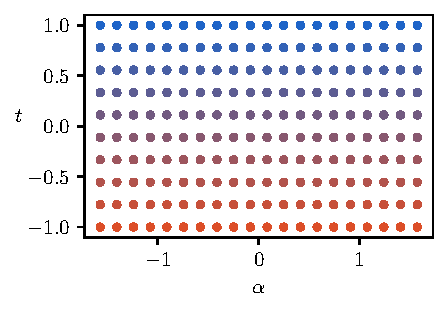
\includegraphics[scale=.75]{img/chapter3/on_disc/disc_original.pdf}%
    \end{minipage}\begin{minipage}{.05\textwidth}\begin{center}
        \Large $ \xrightarrow{T} $
      \end{center}
    \end{minipage}\begin{minipage}{.42\textwidth}\centering
      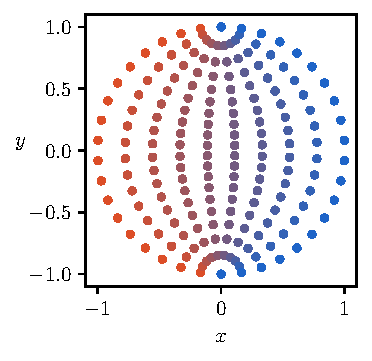
\includegraphics[scale=.75]{img/chapter3/on_disc/disc_transformed.pdf}
    \end{minipage}
  \end{center}
  \caption{The transformation $T(\alpha, t)$ from \eqref{equ:c3_disc_transformation} is applied to a grid of points.}
  \label{fig:c3_disc_transformation}
\end{figure}

To demonstrate the effectiveness of theorem \ref{lem:c3_eigenvalues_curves}, we will consider the family of continuous subdomains
$$
  \Omega_\epsilon = \left\{T(\alpha, t) \,\middle|\, \forall \alpha \in \left[-\frac{\pi}{2}, \frac{\pi}{2}\right], \forall t \in [-1, 2\epsilon - 1]  \right\}\text{.}
$$
On each of these subdomains $\Omega_\epsilon$, we will approximate the eigenvalues of the Schrödinger equation with zero potential:
\begin{equation}\label{equ:c3_disc_schrodinger}
  -\nabla^2 \psi(x, y) = \lambda \psi(x, y)\text{.}
\end{equation}
As boundary conditions we impose $\psi(x, y) = 0$ on the boundary $\dOmega_\epsilon$.

Later on, the found approximate eigenvalues can be compared to the eigenvalues on the unit disc $\Omega_1$, as described in section \ref{sec:c3_standing_waves_on_disc}. Theorem \ref{the:c3_counting_eigenvalues} promises that for an eigenvalue $\lambda_i$ on the unit disc, exactly $i$ moon-shaped subdomains can be found on which this $\lambda_i$ is also an eigenvalue.

\paragraph{Transforming the problem onto a rectangular domain}

Approximating solutions for the eigenvalues of \eqref{equ:c3_disc_schrodinger} on such an exotic domain $\Omega_\epsilon$ is not a trivial task. In principle, this problem could be seen as solving the Schrödinger equation on $[-1,1]^2$ with the potential
$$
  V(x, y) = \begin{cases}
    0       & \text{if $(x, y)\in \Omega_\epsilon$} \\
    +\infty & \text{otherwise}
  \end{cases} {}\text{.}
$$
But numerically, this does not make the problem easier. Yes, the rectangular domain would allow us to employ the earlier developed method. But on the other hand, the potential becomes infinite, which is very difficult to implement with sufficiently high accuracies. Also, Ixaru's method has difficulties with non-continuous potentials. Note: the inability to tackle non-continuous problems is a phenomenon present in many high order numerical methods. In section \ref{sec:c2_experiment_with_jumps}, we have seen that with one-dimensional problems, \matslise{} can avoid these issues by smartly choosing its piecewise approximation. For higher dimensional problems, these kinds of tricks are no longer possible.

We propose another technique. We can transform equation \eqref{equ:c3_disc_schrodinger} from these moon-shaped domains to a more manageable rectangular domain. The cost of this transformation is that \eqref{equ:c3_disc_schrodinger} will no longer be a Schrödinger equation.

As earlier stated, the transformation we will apply is the function $(x, y) = T(\alpha, t)$ from \eqref{equ:c3_disc_transformation}. To formalize this, we introduce $\phi(\alpha, t)$ as
$$
  \phi(\alpha, t) = \psi(T(\alpha, t))\text{.}
$$
With this transformation the Schrödinger equation \eqref{equ:c3_disc_schrodinger} transforms into
\begin{equation}\label{equ:c3_disc_schrodinger_transformed}
  -\mathcal{D}\phi(\alpha, t) = \lambda\phi(\alpha, t)
\end{equation}
with $\phi(\alpha, t)$ defined on the domain $\Xi_\epsilon = \left[-\frac{\pi}{2}, \frac{\pi}{2}\right] \times [-1, 2\epsilon - 1]$. Note that $T(\Xi_\epsilon) = \Omega_\epsilon$. As boundary conditions we impose $\phi(\alpha, t) = 0$ if $(\alpha, t) \in \partial\Xi_\epsilon$. In this expression $\mathcal{D}$ is the differential operator corresponding to $\nabla^2\psi(x, y)$. Calculating this operator by hand is tedious, therefore we will use \sage to do the symbolic heavy lifting for us. To be able to work with the operator $\mathcal{D}$, we first need a procedure to compute it. To ease notation we will denote $T(\alpha, t) = (T^{x}(\alpha, t), T^{y}(\alpha, t))$, and omit the arguments to the functions $\phi$, $\psi$ and $T$. Derivatives will be denoted as $\phi_\alpha = \pdv[]{\phi}{\alpha}$ and $\phi_{\alpha\alpha} = \pdv[2]{\phi}{\alpha}$. We compute all first and second derivatives of $\phi(\alpha, t)$.
\begin{equation}\label{equ:disc_transformation_derivatives}
  \begin{cases}
    \phi_\alpha = \psi_x T^x_\alpha + \psi_y T^y_\alpha                                                                                                                   \\
    \phi_t = \psi_x T^x_t + \psi_y T^y_t                                                                                                                                  \\
    \phi_{\alpha\alpha} = \psi_x T^x_{\alpha\alpha} + \psi_y T^y_{\alpha\alpha} + \psi_{xx} (T^x_\alpha)^2 + 2 \psi_{xy} T^x_\alpha T^y_\alpha + \psi_{yy} (T^y_\alpha)^2 \\
    \phi_{\alpha t} = \psi_x T^x_{\alpha t} + \psi_y T^y_{\alpha t} + \psi_{xx} (T^x_\alpha)(T^x_t) + \psi_{xy} \left(T^x_\alpha T^y_t + T^x_t T^y_\alpha \right)         \\
    \quad\quad\quad\quad {} + \psi_{yy} (T^y_\alpha)(T^y_t)                                                                                                               \\
    \phi_{tt} = \psi_x T^x_{tt} + \psi_y T^y_{tt} + \psi_{xx} (T^x_t)^2 + 2 \psi_{xy} T^x_t T^y_t + \psi_{yy} (T^y_t)^2
  \end{cases}
\end{equation}

The question now is, can we isolate $\psi_{xx} + \psi_{yy}$ from the right-hand side of the system from \eqref{equ:disc_transformation_derivatives}? As this is a linear system in the derivatives of $\psi$, there is a unique linear combination $\vb{c}(\alpha, t) = (c^\alpha, c^t, c^{\alpha\alpha}, c^{\alpha t}, c^{tt})$ of rows such that:
$$
  c^\alpha \phi_\alpha + c^t\phi_t + c^{\alpha\alpha}\phi_{\alpha\alpha} + c^{\alpha t} \phi_{\alpha t} + c^{tt} \phi_{tt} = \psi_{xx} + \psi_{yy}\text{.}
$$

This linear combination allows us to finally determine the operator $\mathcal{D}$, and by extension the partial differential equation \eqref{equ:c3_disc_schrodinger} transforms into. Note that because $\vb{c}$ is dependent on $\alpha$ and $t$, that the operator $\mathcal{D}$ has this dependency as well.
$$
  \mathcal{D} = c^\alpha {\pdv[]{}{\alpha}} + c^t \pdv[]{}{t} + c^{\alpha\alpha} \pdv[]{}{\alpha\alpha} + c^{\alpha t} \pdv[]{}{\alpha t} + c^{tt} \pdv[]{}{tt}
$$

\paragraph{A specialized numerical method}

Before we can analyze eigenvalues of \eqref{equ:c3_disc_schrodinger} or after transformation of the operator $-\mathcal{D}$ in relation to the domain $\Omega_\epsilon$, we still need a method to approximate these eigenvalues. For general partial differential equations with boundary conditions some standard techniques are available, \cite[Chapter~11]{heath_scientific_2002} contains an overview of some of these methods. Our choices include, but are not limited to a finite difference method, or a finite element method or a semidiscrete method with shooting. For our purposes a method which is easy to implement, yet gives reliable results will be the best choice. A simple finite difference scheme will be sufficient.

We will place an $n_\alpha \times n_t$ grid on the domain $\Xi_\epsilon$. This gives rise to the equidistant points $-\frac{\pi}{2}=\alpha_0, \alpha_1, \dots, \alpha_{n_\alpha} = \frac{\pi}{2}$, and the points $-1 = t_0, t_1, \dots t_{n_t} = 1 - 2\epsilon$. The distances between two points are given by $h_\alpha = \frac{\pi}{n_\alpha}$ and $h_t = \frac{2\epsilon}{n_t}$. Because of the homogeneous Dirichlet boundary conditions $\phi_{0,j} = \phi_{n_\alpha,j} = \phi_{i, 0} = \phi_{i,n_t} = 0$ for all $i$ and $j$. These grid points allow us to write down approximations of first and second derivatives of $\phi(\alpha, t)$ in each of the grid points $\phi_{i, j} = \phi(\alpha_i, t_j)$.
\begin{align*}
  {\pdv[]{\phi}{\alpha}}(\alpha_i, t_j)    & = \frac{1}{2h_\alpha}\left( \phi_{i+1,j} - \phi_{i-1,j} \right)                                           \\
  {\pdv[]{\phi}{t}}(\alpha_i, t_j)         & = \frac{1}{2h_t}\left( \phi_{i,j+1} - \phi_{i,j-1} \right)                                                \\
  {\pdv[2]{\phi}{\alpha}}(\alpha_i, t_j)   & = \frac{1}{h_\alpha^2}\left( \phi_{i+1,j} - 2 \phi_{i,j} + \phi_{i-1,j} \right)                           \\
  {\pdv[]{\phi}{\alpha}{t}}(\alpha_i, t_j) & = \frac{1}{4h_\alpha h_t}\left( \phi_{i+1,j+1} - \phi_{i+1,j-1} - \phi_{i-1,j+1} + \phi_{i-1,j-1} \right) \\
  {\pdv[2]{\phi}{t}}(\alpha_i, t_j)        & = \frac{1}{h_t^2}\left( \phi_{i,j+1} - 2 \phi_{i,j} + \phi_{i,j-1} \right)
\end{align*}

When working with finite difference schemes, especially for a more  advanced operator such as $\mathcal{D}$, writing out all formulas becomes quite tedious. Therefore, it is much more comprehensive if we introduce some matrix notation. Let us denote the identity matrix of dimensions $n \times n$ as $\vb{I}_n$. Furthermore, a diagonal matrix with $a_1, \dots a_n$ on the diagonal will be denoted as $\diag_n(a_1, \dots, a_n)$, and an $n \times n$ tridiagonal Toeplitz matrix, with $c_{0}$ on the main diagonal, $c_{-1}$ below it and $c_1$ above it, will be denoted as $\tridiag_{n}(c_{-1}, c_{0}, c_1)$. To aid the finite difference approximations we introduce $\vb{D}^{(1)}_n = \frac{1}{2}\tridiag_n(-1,0,1)$ and $\vb{D}^{(2)}_n = \tridiag_n(1,-2,1)$

We will define the Kronecker product of a $k \times l$ matrix $\vb{A}$ and $m \times n$ matrix $\vb{B}$ as the $km \times ln$ block matrix:
$$
  \vb{A} \otimes \vb{B} := \begin{pmatrix}
    A_{1,1} \vb{B} & A_{1, 2} \vb{B} & \dots  & A_{1, l} \vb{B} \\
    A_{2,1} \vb{B} & A_{2, 2} \vb{B} & \dots  & A_{2, l} \vb{B} \\
    \vdots         & \vdots          & \ddots & \vdots          \\
    A_{k,1} \vb{B} & A_{k, 2} \vb{B} & \dots  & A_{k, l} \vb{B} \\
  \end{pmatrix}{}\text{.}
$$

To approximate \eqref{equ:c3_disc_schrodinger_transformed} as a matrix problem, we need to aggregate the grid points $\phi_{i,j}$ as a vector. For this we define
$$
  \vb*{\phi} := \transpose{\begin{pmatrix}
      \phi_{1,1} & \phi_{2,1} & \dots & \phi_{n_\alpha-1, 1} & \phi_{1,2} & \dots & \phi_{n_\alpha-1, n_t-1}
    \end{pmatrix}}\text{.}
$$
Also, to be able to write down $\mathcal{D}$ as a matrix operation we need to define
$$
  \vb{C}^{t} := \diag{\begin{pmatrix}
      c^{t}(\alpha_1, t_1) & \dots & c^{t}(\alpha_{n_\alpha-1}, t_1) & c^{t}(\alpha_1, t_2) & \dots & c^{t}(\alpha_{n_\alpha-1}, t_{n_t-1})
    \end{pmatrix}}\text{,}
$$
and analogous for $\vb{C}^{\alpha}$, $\vb{C}^{\alpha\alpha}$, $\vb{C}^{\alpha t}$ and $\vb{C}^{t t}$.

All this notation allows us to approximate \eqref{equ:c3_disc_schrodinger_transformed} as a matrix eigenvalue problem:
$$
  -\vb{M} \vb*{\phi} = \lambda \vb*{\phi}
$$
with
\begin{align*}
  \vb{M} = {} & \frac{1}{h_\alpha} \vb{C}^{\alpha} \left(\vb{I}_{n_t - 1}\otimes \vb{D}^{(1)}_{n_\alpha - 1} \right) + \frac{1}{h_t} \vb{C}^{t} \left(\vb{D}^{(1)}_{n_t - 1}  \otimes \vb{I}_{n_\alpha - 1}\right)                \\
              & {} + \frac{1}{h_\alpha^2} \vb{C}^{\alpha\alpha} \left(\vb{I}_{n_t - 1}\otimes \vb{D}^{(2)}_{n_\alpha - 1}\right) + \frac{1}{h_t^2} \vb{C}^{tt} \left(\vb{D}^{(2)}_{n_t - 1}  \otimes \vb{I}_{n_\alpha - 1}\right) \\
              & {} + \frac{1}{h_\alpha h_t} \vb{C}^{\alpha t} \left(\vb{I}_{n_t - 1}\otimes \vb{D}^{(1)}_{n_\alpha - 1} \right) \left( \vb{D}^{(1)}_{n_t - 1}  \otimes \vb{I}_{n_\alpha - 1} \right)\text{.}
\end{align*}

\begin{figure}
  \begin{center}
    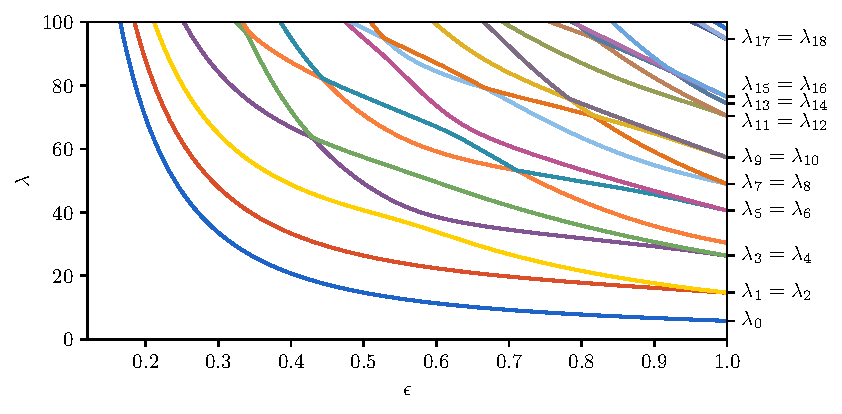
\includegraphics[width=\textwidth]{img/chapter3/on_disc/eigenvalues_flow.pdf}
    \caption{Eigenvalues in relation to $\epsilon$.}
    \label{fig:c3_disc_eigenvalues_flow}
  \end{center}
\end{figure}

\paragraph{Analysis of eigenvalues in relation to the domain}

With a numerical method to compute eigenvalues of the wave equation \eqref{equ:c3_disc_schrodinger} on moon-shaped domains $\Omega_\epsilon$, and a comprehensive analysis of the true eigenvalues of this equation on the disc $\Omega_1$, we are able to demonstrate theorem \ref{lem:c3_eigenvalues_curves}.

By employing our numerical method on different domains $\Omega_\epsilon$ we can compute figure \ref{fig:c3_disc_eigenvalues_flow}. Here each line corresponds to a different eigenvalue. The lowest blue line visualizes the changes in the lowest eigenvalue according to the domain. For small domains $\epsilon \to 0$, this value becomes larger. The red line, right above the blue line corresponds to the eigenvalue with index $1$ of the wave equation on $\Omega_\epsilon$. For $\Omega_1$, this eigenvalue has a double multiplicity $\lambda_1 = \lambda_2$. But for all smaller domains, this degeneracy disappears, and $\lambda_1$ is a single eigenvalue. Which eigenvalue each line represent is marked on the right side. In accordance with theorem \ref{lem:c3_eigenvalues_curves} all lines in figure \ref{fig:c3_disc_eigenvalues_flow} are continuous, decreasing and unbounded when $\epsilon \to 0$.


\begin{figure}
  \begin{center}
    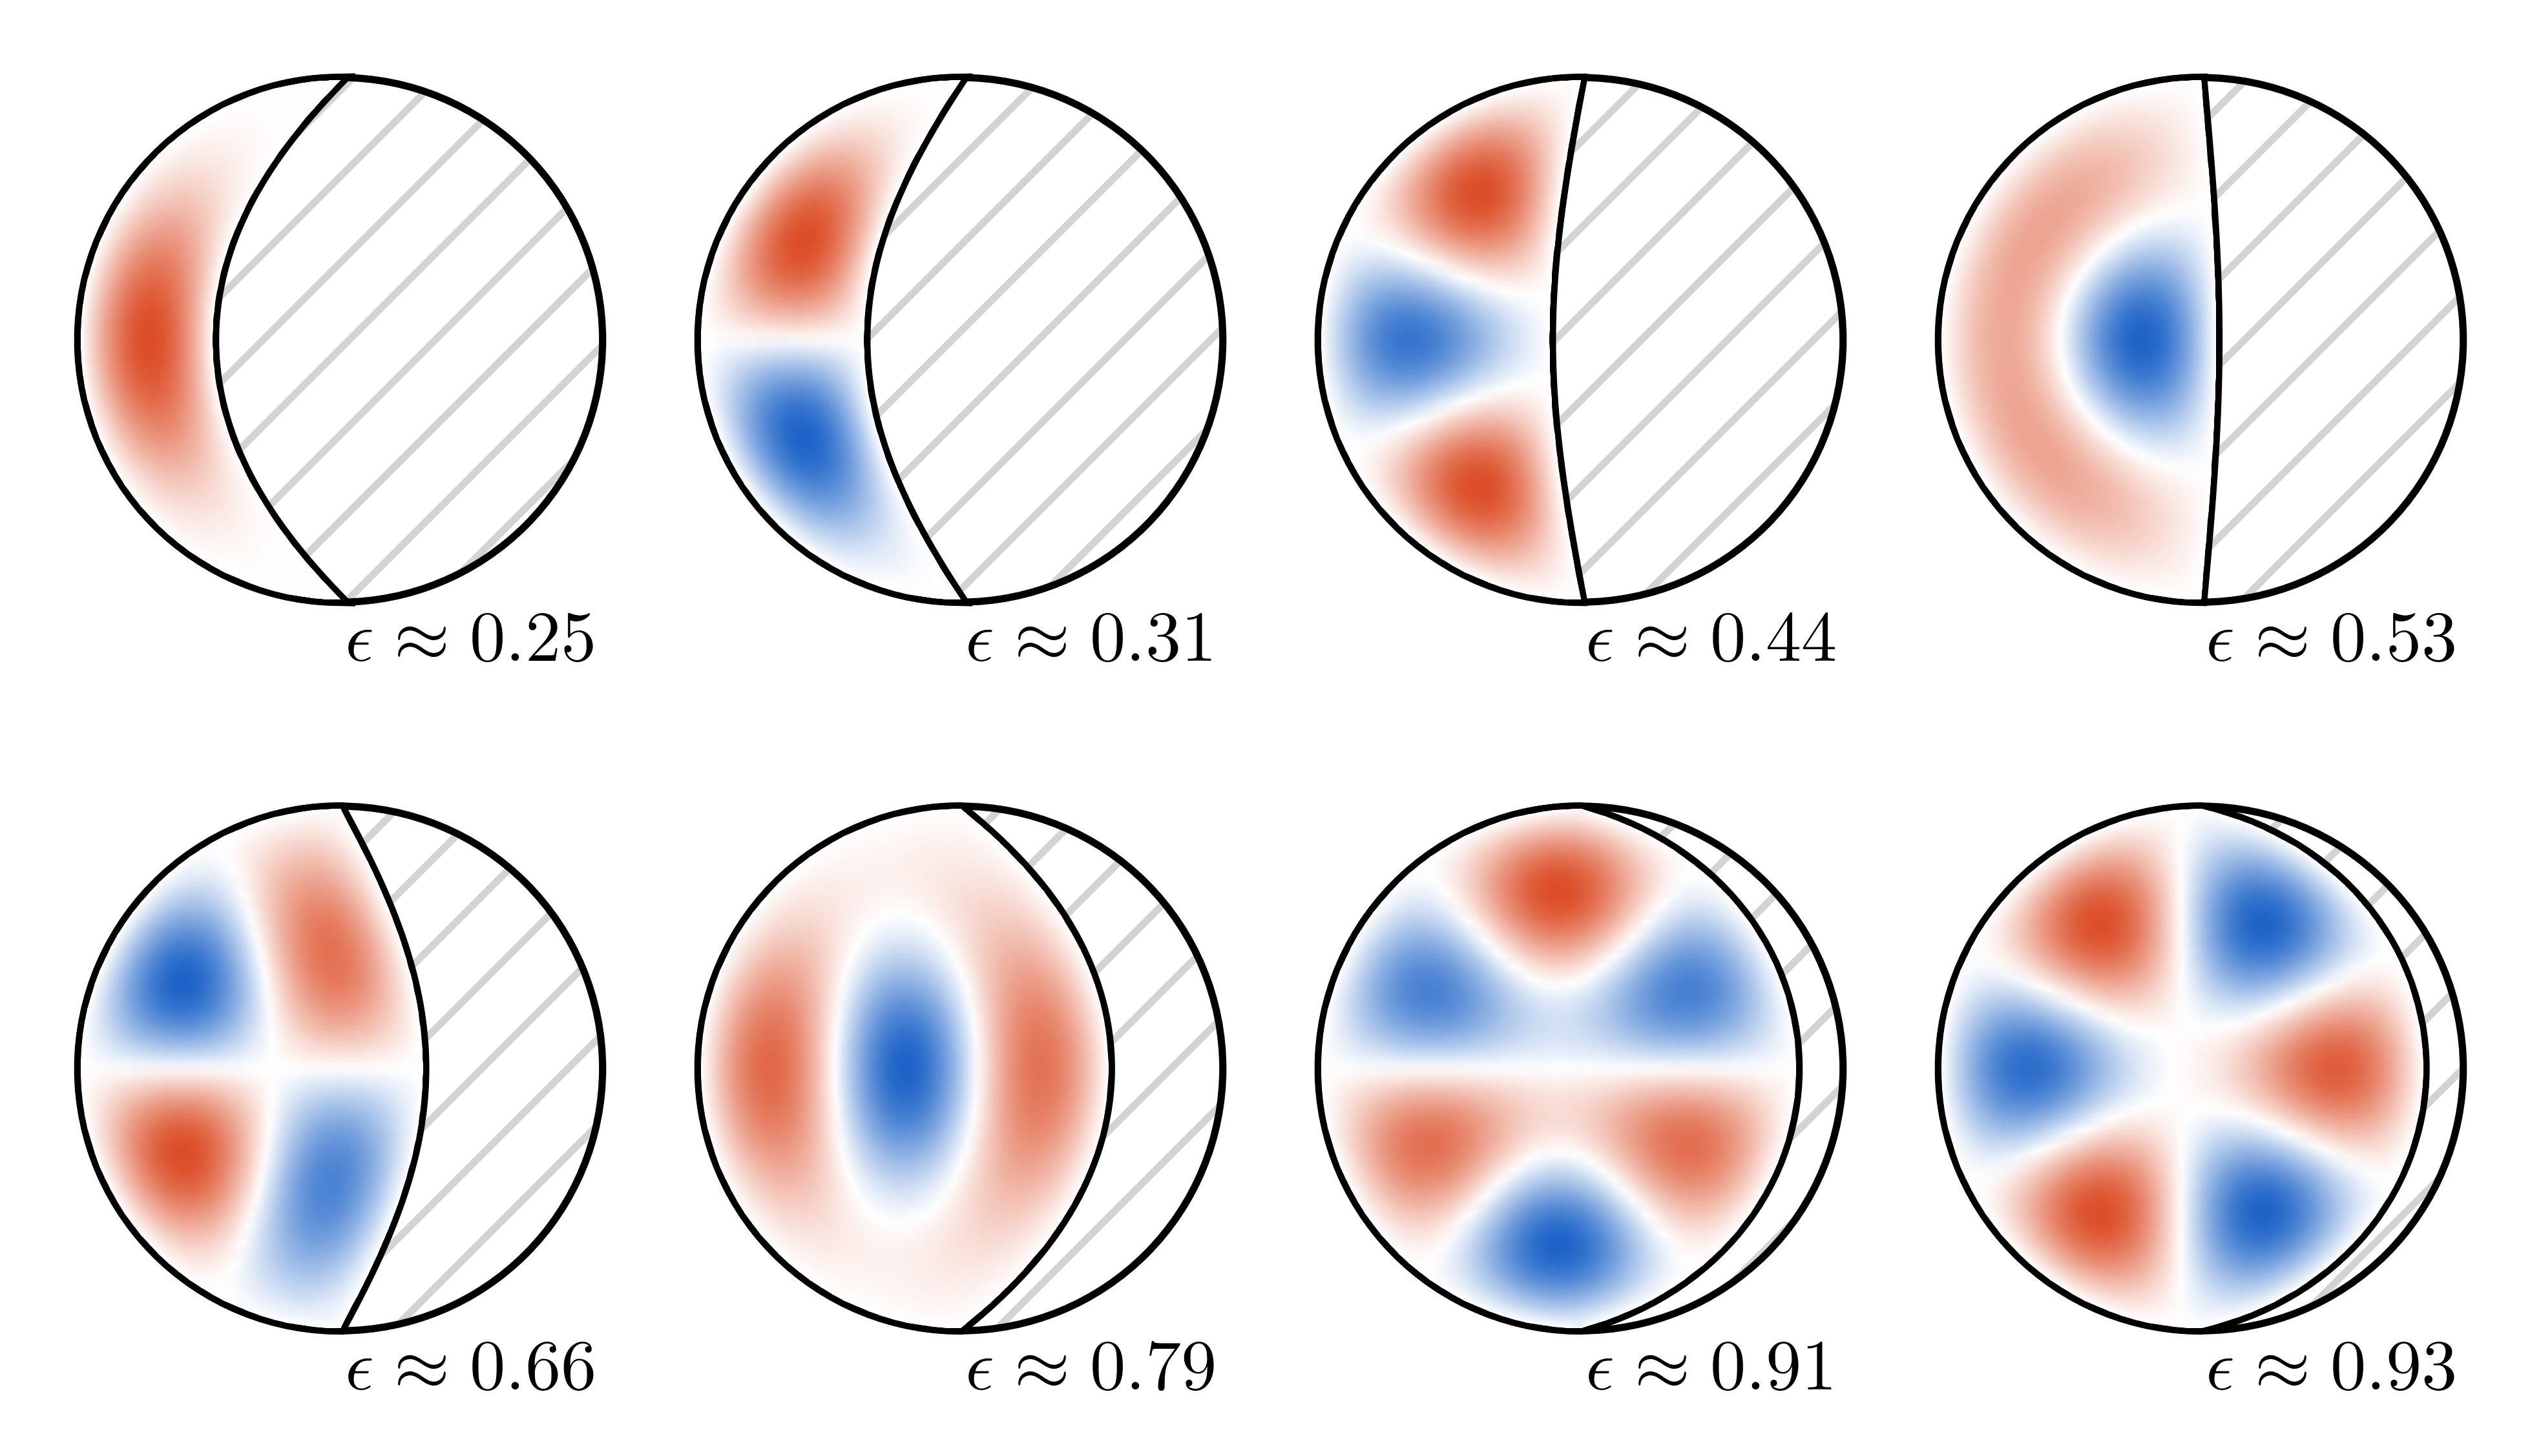
\includegraphics[width=\textwidth]{img/chapter3/on_disc/solutions.png}
    \caption{There are $8$ smaller moon shaped domains on which $\lambda = 45$ is an eigenvalue of the wave equation $-\nabla^2 \psi = \lambda \psi$ with homogeneous Dirichlet boundary conditions.}
    \label{fig:c3_disc_solutions}
  \end{center}
\end{figure}


Consider now the fixed value of $E = 45$. From the analysis in \ref{sec:c3_standing_waves_on_disc} we know that there are $8$ eigenvalues, counted with multiplicity, less than $E$. This means, following theorem \ref{the:c3_counting_eigenvalues}, there should be exactly $8$ moon shaped domains on which $E$ is also an eigenvalue. These eight domains, with the corresponding eigenfunction of $E = 45$, are plotted in figure \ref{fig:c3_disc_solutions}.

\section{Numerical experiments}\label{sec:c3_experiments}

\subsection{Ixaru's potential}\label{sec:c3_experiment_ixaru}

\todo{Copy from article}

\subsection{Hénon-Heiles}\label{sec:c3_experiment_henon}

\todo{Copy from article}

\section{Conclusions}


\todo{}

\begin{enumerate}
  \item accuracy
  \item run time
  \item numerical stability
  \item order estimates
  \item benefits vs. disadvantages
  \item possible future work
\end{enumerate}


\stopchapter
